\documentclass[11pt]{amsart}
\usepackage{amsmath,amssymb,amsthm,mathtools}
\usepackage[margin=1in]{geometry}
\usepackage{booktabs}
\usepackage{longtable}
\usepackage{hyperref}
\usepackage{graphicx}
\usepackage{xcolor}
\usepackage{enumitem}
\usepackage{tikz-cd}

\newtheorem{theorem}{Theorem}[section]
\newtheorem{conjecture}[theorem]{Conjecture}
\newtheorem{proposition}[theorem]{Proposition}
\newtheorem{lemma}[theorem]{Lemma}
\newtheorem{corollary}[theorem]{Corollary}
\theoremstyle{definition}
\newtheorem{definition}[theorem]{Definition}
\theoremstyle{remark}
\newtheorem{remark}[theorem]{Remark}

\title[The Critical Line: A Survey]{The Critical Line: A Survey of Recent Progress on the Riemann Hypothesis}
\author{David Alejandro Trejo Pizzo}
\thanks{Independent Researcher. \texttt{dtrejopizzo@gmail.com}}

\begin{document}
\begin{abstract}
The Riemann Hypothesis (RH), asserting that all non-trivial zeros of the Riemann zeta function $\zeta(s)$ lie on the critical line $\operatorname{Re}(s) = 1/2$, remains the central open problem in analytic number theory. This survey examines recent progress across three principal directions of attack: the \textbf{analytic approach}, where the 2024 breakthrough of Guth and Maynard synthesizes additive combinatorics and time-frequency geometry to yield the first improvement to zero density estimates near $\sigma = 3/4$ in over eighty years; the \textbf{spectral approach}, where the physical constraints of unitarity in conformal field theory and the localization of prolate wave operators provide new rigid frameworks for the absorption spectrum; and the \textbf{algebro-geometric approach}, where the program of Connes and Consani seeks to formalize a Riemann--Roch theorem and intersection theory over the sphere spectrum $\mathbb{S}$ as an absolute base.

We provide detailed technical accounts of these developments, evaluate the arithmetic teeth of the proposed geometric models, and assess the principal conceptual obstacles that remain. Ultimately, we identify a striking theoretical convergence: across analytic, spectral, and geometric boundaries, the resolution of the Riemann Hypothesis appears in each case to reduce to establishing a foundational \textbf{positivity} condition---suggestive of a deeper, possibly unified positivity principle, though the positivities in question live in very different mathematical categories and are not yet known to be equivalent.
\end{abstract}
\maketitle

\tableofcontents
\newpage

%% ======================================================================
\section{Introduction and Historical Context}\label{sec:intro}
%% ======================================================================

The Riemann zeta function, defined for $\operatorname{Re}(s) > 1$ by the Dirichlet series
\[
\zeta(s) = \sum_{n=1}^{\infty} n^{-s} = \prod_{p \text{ prime}} (1 - p^{-s})^{-1},
\]
admits a meromorphic continuation to the entire complex plane with a simple pole at $s = 1$. The Euler product relates the analytic properties of $\zeta(s)$ to the distribution of prime numbers. The \emph{non-trivial zeros}---those in the critical strip $0 < \operatorname{Re}(s) < 1$---govern the error term in the Prime Number Theorem and, more broadly, encode the fine structure of the primes.

\begin{conjecture}[Riemann, 1859]\label{conj:rh}
All non-trivial zeros of $\zeta(s)$ satisfy $\operatorname{Re}(s) = 1/2$.
\end{conjecture}

Riemann stated this conjecture in his celebrated 1859 memoir \cite{riemann1859}, noting that it was ``very probable'' (sehr wahrscheinlich) but that he had set it aside after a few brief unsuccessful attempts. The conjecture was included by Hilbert as the eighth of his 23 problems in 1900 and by the Clay Mathematics Institute as one of the seven Millennium Prize Problems in 2000 \cite{bombieri2000}.

\subsection{Consequences of the Riemann Hypothesis}\label{sec:consequences}

Before discussing progress toward a proof, we briefly indicate why RH is important. Its consequences pervade number theory and beyond:
\begin{itemize}
\item \textbf{Prime distribution.} RH implies the best possible error term in the Prime Number Theorem: $\pi(x) = \operatorname{Li}(x) + O(\sqrt{x}\log x)$, where $\operatorname{Li}(x) = \int_2^x dt/\log t$. Without RH, the best known error term is exponentially worse.
\item \textbf{Primes in short intervals.} RH implies that the interval $[x, x + C\sqrt{x}\log x]$ contains a prime for all sufficiently large $x$ and an appropriate constant $C$.
\item \textbf{Arithmetic functions.} RH implies sharp bounds for the summatory function of the M\"obius function: $\sum_{n \le x} \mu(n) = O(x^{1/2+\varepsilon})$, and for many other arithmetic functions.
\item \textbf{The Generalized Riemann Hypothesis} (GRH) for Dirichlet $L$-functions has consequences for the distribution of primes in arithmetic progressions, the least quadratic residue, and the efficiency of primality testing algorithms (the Miller--Rabin test is deterministic under GRH).
\end{itemize}

\subsection{What is Known Unconditionally}\label{sec:known}

To orient the reader, we summarize the principal unconditional results concerning the zeros:
\begin{enumerate}[label=(\roman*)]
\item \textbf{Infinitely many zeros on the line.} Hardy (1914) \cite{hardy1914} proved that $\zeta(1/2 + it) = 0$ for infinitely many real $t$.
\item \textbf{A positive proportion.} Selberg \cite{selberg1942} proved that a positive proportion of the zeros lie on the critical line, and quantitative lower bounds have been successively improved (Section~\ref{sec:proportion}).
\item \textbf{Zero-free regions.} The zeta function has no zeros in explicit regions near $\operatorname{Re}(s) = 1$ (Section~\ref{sec:zfr}).
\item \textbf{Density estimates.} The number of zeros off the critical line satisfies strong quantitative bounds (Section~\ref{sec:gm}).
\item \textbf{Computational verification.} RH has been rigorously verified for the first $1.3 \times 10^{13}$ non-trivial zeros, corresponding to heights up to $T \approx 3 \times 10^{12}$ (Platt--Trudgian; Section~\ref{sec:verification}).
\end{enumerate}
No unconditional result excludes the existence of even a single zero off the critical line.

\subsection{The Function Field Analogue}\label{sec:ff-intro}

The Riemann Hypothesis is a theorem in the function field setting. For a smooth projective curve $C$ of genus $g$ over $\mathbb{F}_q$, the zeta function $Z(C/\mathbb{F}_q, T)$ is a rational function whose zeros all satisfy $|T| = q^{-1/2}$ (equivalently, the reciprocal roots of the numerator have absolute value $q^{1/2}$). This was proved by Weil \cite{weil1948} using the intersection theory of $C \times C$, and generalized by Deligne \cite{deligne1974} to arbitrary varieties. The existence of a proof in the function field case is both a source of optimism (the statement is true in an analogous setting) and a guide for strategy (the geometric methods that work there might be adapted to $\mathbb{Z}$).

\subsection{Organization of This Survey}

We organize the presentation around three principal directions of attack. Section~\ref{sec:analytic} covers the analytic approach: zero-free regions, zero density estimates (including the 2024 Guth--Maynard breakthrough), the proportion of zeros on the critical line, and extremal behavior via resonance methods and log-correlated fields. Section~\ref{sec:comp} discusses computational verification and the statistical properties of the zeros, including the GUE connection. Section~\ref{sec:spectral} treats the spectral approach: the Hilbert--P\'olya conjecture, the Berry--Keating Hamiltonian, the Montgomery pair correlation conjecture, Connes' trace formula, and the scalar modular bootstrap. Section~\ref{sec:geometric} covers the algebro-geometric approach via $\mathbb{F}_1$-geometry and the Connes--Consani program. Section~\ref{sec:equiv} discusses equivalent reformulations, including Li's criterion, Voronin universality, and the structural role of the Euler product. We conclude with a synthesis and assessment of future prospects.

For comprehensive introductions to the Riemann Hypothesis, we refer to the books of Edwards \cite{edwards1974} and Titchmarsh \cite{titchmarsh1986}, the survey of Conrey \cite{conrey2003}, and the Clay Mathematics Institute problem statements of Bombieri \cite{bombieri2000} and Sarnak \cite{sarnak2004}. For a recent perspective situating the problem in historical and contemporary context, see the essay of Connes \cite{connes2026}.

%% ======================================================================
\section{The Analytic Front: Quantitative Constraints on Zero Distribution}\label{sec:analytic}
%% ======================================================================

The analytic approach to the Riemann Hypothesis seeks to constrain the location and density of zeros of $\zeta(s)$ through estimates on exponential sums, mean values, and the growth of $\zeta(s)$ in the critical strip. While this approach has not yet produced a structural explanation for the truth of RH, it provides the strongest unconditional quantitative information currently available.

For general background on the analytic theory, we refer to the monographs of Titchmarsh \cite{titchmarsh1986} and Iwaniec--Kowalski \cite{iwaniec2004}, and the survey of Conrey \cite{conrey2003}.

\begin{figure}[h!]
\centering
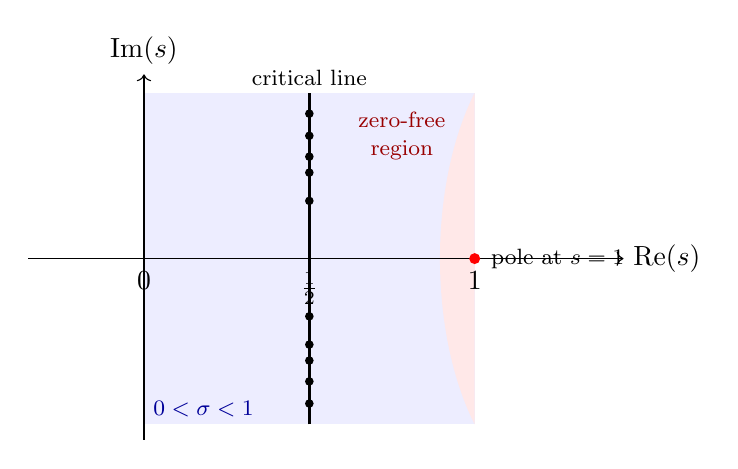
\begin{tikzpicture}[xscale=4.2,yscale=0.78]
    % critical strip
    \fill[blue!7] (0,-2.7) rectangle (1,2.7);
    % zero-free region (schematic sliver hugging Re=1, narrowing with height)
    \fill[red!9]
        (1,-2.7) .. controls (0.86,-1.2) and (0.86,1.2) .. (1,2.7) -- (1,-2.7);
    % axes
    \draw[->] (-0.35,0)--(1.45,0) node[right]{$\operatorname{Re}(s)$};
    \draw[->] (0,-2.95)--(0,3.0) node[above]{$\operatorname{Im}(s)$};
    \foreach \x/\lab in {0/0,0.5/{\tfrac12},1/1} \draw (\x,0.06)--(\x,-0.06) node[below]{$\lab$};
    % critical line
    \draw[very thick] (0.5,-2.7)--(0.5,2.7);
    \node[fill=white,inner sep=1pt] at (0.5,2.95) {\footnotesize critical line};
    % sample zeros on the line
    \foreach \y in {0.94,1.40,1.66,2.00,2.36,-0.94,-1.40,-1.66,-2.00,-2.36}
        \node[circle,fill,inner sep=1.1pt] at (0.5,\y){};
    % pole
    \node[circle,fill=red,inner sep=1.4pt] at (1,0){};
    \node[right] at (1.02,0.0){\footnotesize pole at $s=1$};
    % labels
    \node[blue!60!black] at (0.18,-2.45){\footnotesize $0<\sigma<1$};
    \node[red!60!black,align=center] at (0.78,2.0){\footnotesize zero-free\\[-2pt]\footnotesize region};
\end{tikzpicture}
\caption{The critical strip $0<\operatorname{Re}(s)<1$ (shaded blue). The Riemann Hypothesis asserts that every non-trivial zero (dots) lies on the critical line $\operatorname{Re}(s)=\tfrac12$. Classical zero-free regions (shaded red) hug the edge $\operatorname{Re}(s)=1$ and narrow as $|\operatorname{Im}(s)|$ grows (Section~\ref{sec:zfr}); $\zeta$ has a simple pole at $s=1$.}
\label{fig:strip}
\end{figure}

%% ----------------------------------------------------------------------
\subsection{Zero-Free Regions: The Quantitative Boundary}\label{sec:zfr}
%% ----------------------------------------------------------------------

It is known unconditionally that $\zeta(s)$ has no zeros in a region of the form $\sigma \ge 1 - f(t)$ for an explicit function $f(t) \to 0$ as $t \to \infty$. The boundary of this zero-free region represents the limit of current analytic methods.

The classical zero-free region, established by de la Vall\'ee Poussin \cite{delavallee1899} in 1899 as a consequence of his proof of the Prime Number Theorem, takes the form $\sigma \ge 1 - c/\log|t|$ for an absolute constant $c > 0$. This remains the best result for ``small'' $|t|$ and is the form most directly relevant to explicit estimates in prime number theory.

For large $|t|$, the Korobov--Vinogradov method \cite{korobov1958} (1958) improved the asymptotic shape to
\[
\sigma \ge 1 - \frac{c}{(\log|t|)^{2/3}(\log\log|t|)^{1/3}},
\]
which remains the best known. The improvement over de la Vall\'ee Poussin arises from Vinogradov's method of estimating exponential sums, which exploits the multiplicative structure of the integers more deeply than the classical approach. Progress since 1958 has consisted of improving the explicit constants rather than the exponents.

The proof of zero-free regions relies on the non-vanishing of $\zeta(s)$ near $\operatorname{Re}(s) = 1$, which is established by a positivity argument. The classical method uses the inequality
\[
3 + 4\cos\theta + \cos 2\theta = 2(1 + \cos\theta)^2 \ge 0
\]
to show that $\operatorname{Re}[3\log\zeta(\sigma) + 4\log\zeta(\sigma+it) + \log\zeta(\sigma+2it)] \ge 0$ for $\sigma > 1$, which forces $\zeta(\sigma + it) \neq 0$ in a region near $\sigma = 1$. Improvements come from using more general trigonometric polynomials $\sum_{k=0}^{K} a_k \cos(k\theta) \ge 0$ with optimized coefficients $a_k$ (subject to $a_0 < 2a_1$, which is the condition that excludes the line $\sigma = 1$ itself).

In January 2024, \textbf{Mossinghoff, Trudgian, and Yang} \cite{mossinghoff2024} published the most significant refinement of these explicit bounds in decades. They systematically optimized these trigonometric polynomial coefficients using linear programming, and incorporated the rigorous computational verification of zeros at large heights (specifically, the Platt--Trudgian result \cite{platt2021}) to handle the ``low height'' regime separately. Their principal results are summarized in Table~\ref{tab:zfr}.

\begin{table}[h!]
    \centering
    \caption{Explicit zero-free regions for $\zeta(s)$ (Mossinghoff--Trudgian--Yang, 2024).}\label{tab:zfr}
    \vspace{0.2cm}
    \begin{tabular}{@{}p{3.5cm}p{5cm}p{3cm}p{3.5cm}@{}}
        \toprule
        \textbf{Region Type} & \textbf{Form} ($\sigma \ge \dots$) & \textbf{Key Constants} & \textbf{Remarks} \\
        \midrule
        Korobov--Vinogradov & $1 - \frac{1}{C (\log |t|)^{2/3} (\log \log |t|)^{1/3}}$ & $C = 55.241$ for $|t| \ge 3$ & Best asymptotic form. The exponent $2/3$ remains a fundamental barrier. \\
        \midrule
        De la Vall\'ee Poussin & $1 - \frac{1}{C \log |t|}$ & $C = 5.558691$ for $|t| \ge 2$ & Relevant for explicit prime counting estimates. \\
        \midrule
        Improved asymptotic & $1 - \frac{1}{C (\log |t|)^{2/3} (\log \log |t|)^{1/3}}$ & $C = 48.1588$ for $|t|$ suff. large & Better constant for large $|t|$; same exponent $2/3$. \\
        \midrule
        Intermediate & Defined via explicit $h(t)$ & $h(t) = 16427 \log |t| + 7.096$ & Bridges the gap between computational verification and asymptotic bounds. \\
        \bottomrule
    \end{tabular}
\end{table}

\begin{remark}
The exponent $2/3$ in the Korobov--Vinogradov region arises from bounds on exponential sums of the form $\sum n^{it}$ via Vinogradov's method. Despite the resolution of the main conjecture in the Vinogradov Mean Value Theorem by Bourgain--Demeter--Guth \cite{bourgain2016} and Wooley \cite{wooley2016}, this exponent has not been improved in the zero-free region context. This suggests a natural barrier: the exponential sum estimates that feed into the zero-free region argument are already essentially optimal. To prove RH, one would need to extend the zero-free region to $\sigma \ge 1/2 + \varepsilon$ for all $\varepsilon > 0$; the current regions, which narrow logarithmically as $t \to \infty$, are infinitely far from this goal.
\end{remark}

%% ----------------------------------------------------------------------
\subsection{The 2024 Guth--Maynard Breakthrough on Zero Density}\label{sec:gm}
%% ----------------------------------------------------------------------

If the zero-free region cannot be widened substantially with current methods, one may instead ask: how dense can zeros be off the critical line? This is the subject of \textbf{zero density estimates}. Let $N(\sigma, T)$ denote the number of zeros $\rho = \beta + i\gamma$ of $\zeta(s)$ with $\beta \ge \sigma$ and $|\gamma| \le T$. The Riemann Hypothesis asserts $N(\sigma, T) = 0$ for all $\sigma > 1/2$.

The connection between zero density and Dirichlet polynomials is classical: if $\zeta(s)$ has a zero at $\sigma + it$, then a related Dirichlet polynomial $D(t) = \sum_{n \sim N} a_n n^{-it}$ must take an anomalously large value near $t$. Bounding $N(\sigma, T)$ therefore reduces to bounding the Lebesgue measure of the set where Dirichlet polynomials are large.

\subsubsection{The Ingham Barrier and the Fourth Moment Limitation}

In 1940, Ingham \cite{ingham1940} established that $N(3/4, T) \ll T^{3/5 + \varepsilon}$. The exponent $3/5 = 0.60$ proved remarkably resistant to improvement and stood for over eighty years. Subsequent work by Huxley \cite{huxley1972}, Heath-Brown, Jutila, Bourgain, Watt, and others improved the density estimates for various ranges of $\sigma$, but in the critical region near $\sigma = 3/4$---the range most relevant to the prime number theorem in short intervals---the Ingham exponent could not be beaten. Near the edge $\sigma \to 1$, explicit zero density estimates have been refined by Bellotti \cite{bellotti2023}, who obtained sharp explicit bounds applicable to problems in prime number theory.

This barrier was not merely a consequence of unoptimized bounds, but a fundamental structural limitation of the existing methodology. Ingham's approach, and its subsequent refinements, relied fundamentally on bounding the measure of the exceptional set $\{t \in [0,T] : |D(t)| \ge V\}$ by utilizing H\"older's inequality and the fourth moment of $D(t)$. The fourth moment $\int_0^T |D(t)|^4 dt$ translates arithmetically into counting the number of solutions to the Diophantine equation $n_1 n_2 = n_3 n_4$, which relies strictly on identities of divisor sums. This algebraic approach is inherently blind to the fine geometric distribution of the frequencies $\log n$. It treats the interference between terms as relatively unstructured and global. Consequently, the exponent $3/5$ represented the natural absolute limit of what could be deduced from $L^4$-norm estimates without actively exploiting the localized constructive interference of Dirichlet polynomials.

\subsubsection{The Guth--Maynard Method: Decoupling, Wave Packets, and Kakeya}

In May 2024, \textbf{Guth and Maynard} \cite{guth2024} broke the Ingham barrier by completely circumventing the $L^4$ bottleneck. They introduced techniques from continuous harmonic analysis and additive combinatorics into the study of Dirichlet polynomials, synthesizing two distinct mathematical traditions:

\begin{enumerate}[label=(\roman*)]
\item \textbf{$\ell^2$-Decoupling and Time-Frequency Geometry.} The Bourgain--Demeter--Guth theorem \cite{bourgain2016} provides sharp $\ell^2$-decoupling inequalities for hypersurfaces. Guth and Maynard recognized that the exceptional set where $|D(t)| \ge V$ can be analyzed by subdividing the time interval $[0, T]$ into multiple scales. At each scale, the Dirichlet polynomial is locally decomposed into ``wave packets'' that are strictly concentrated on rectangular ``tubes'' in the time-frequency phase space. 

Crucially, this incidence geometry is deeply connected to the Kakeya conjecture. The applicability of the Bourgain--Demeter--Guth decoupling theorem requires the \emph{non-vanishing of curvature} of the frequency manifold: specifically, the phase function $\phi(n) = t \log n$ associated to the Dirichlet polynomial has second derivative $\phi''(n) = -t/n^2 \neq 0$, so the frequencies $n \mapsto \log n$ parametrize a curve with strictly non-zero curvature. This analytic condition ensures that the $\ell^2$-decoupling inequalities rigorously limit how often wave packets pointing in different directions can constructively interfere. The clustering of zeros is geometrically restricted by the capacity of these wave packets to overlap, which is governed by the exact same geometric incidence bounds that control Kakeya sets.

\item \textbf{Efficient Congruencing and Arithmetic Sieve.} Wooley's method of efficient congruencing \cite{wooley2016} provides sharp mean value estimates for exponential sums via a $p$-adic iteration scheme. Guth and Maynard adapt key structural insights from this method---particularly the hierarchical decomposition of the frequency space into major and minor arcs at multiple scales. By understanding how algebraic congruence conditions dictate the spatial clustering of frequencies, they bound the number of overlapping tubes in the major arcs.
\end{enumerate}

\subsubsection{The Vinogradov Mean Value Theorem Connection}

The resolution of the main conjecture in the Vinogradov Mean Value Theorem (VMVT) by Bourgain--Demeter--Guth \cite{bourgain2016} and Wooley \cite{wooley2016} is a crucial prerequisite for this framework. The VMVT provides sharp bounds for the mean value
\begin{equation}
\int_0^1 \cdots \int_0^1 \left| \sum_{n=1}^{N} e(n\alpha_1 + n^2 \alpha_2 + \cdots + n^k \alpha_k) \right|^{2s} \, d\alpha_1 \cdots d\alpha_k,
\end{equation}
where $e(x) = e^{2\pi i x}$. The main conjecture, now a theorem, asserts that this integral is $\ll N^{s+\varepsilon} + N^{2s - k(k+1)/2 + \varepsilon}$. The two proofs---Bourgain--Demeter--Guth via $\ell^2$-decoupling for the moment curve in $\mathbb{R}^k$, and Wooley via $p$-adic efficient congruencing---take fundamentally different approaches but arrive at the same optimal bound. Guth and Maynard synthesize ideas from both traditions: the geometric perspective of decoupling (induction-on-scales and bounding tube overlaps) and the arithmetic structure exploited by efficient congruencing (major arc clustering).

\subsubsection{The Zero Density Result and the Holy Grail}

By optimizing the interplay between the $\ell^2$-decoupling bounds for the continuous variables and the arithmetic sieve bounds for the coefficients $a_n$, the new geometric approach yields a definitive improvement.

\begin{theorem}[Guth--Maynard, 2024]\label{thm:gm}
For $\sigma \ge 3/4$, the zero density estimate satisfies
\begin{equation}\label{eq:gm}
N(\sigma, T) \ll T^{\frac{30(1-\sigma)}{13} + \varepsilon}.
\end{equation}
\end{theorem}

At the critical value $\sigma = 3/4$, the new exponent is $30/52 = 15/26 \approx 0.5769$, which securely bypasses Ingham's rigid barrier of $3/5 = 0.60$. Breaking specific exponents in analytic number theory typically signals the introduction of a genuinely new method. In this case, the barrier that stood for eighty years was an artifact of insufficient geometric understanding of Dirichlet polynomials. The exponent $30(1-\sigma)/13$ quoted here is the form reported in subsequent literature (see, e.g., Hieu \cite{hieu2025} and Tao--Trudgian--Yang \cite{tao2025}); the reader should consult the original preprint \cite{guth2024} for the precise formulation. 

While the exponent $15/26$ establishes a new gold standard for $\sigma \ge 3/4$, the ultimate analytic ``holy grail'' is to extend this geometric incidence framework down to the critical line $\sigma = 1/2$, fully resolving the density hypothesis through the structural control of wave packet intersections.

\subsubsection{Consequences}

\begin{enumerate}[label=(\roman*)]
\item \textbf{Primes in short intervals.} The Guth--Maynard estimate implies the existence of primes in intervals $[x, x + x^{\theta}]$ for $\theta$ smaller than previously achievable. Specifically, the exponent $\theta$ can be strictly reduced below the Huxley record of $7/12 \approx 0.583$ to $\theta = 17/30 \approx 0.567$.

\item \textbf{Density hypothesis.} The \emph{density hypothesis} asserts that $N(\sigma, T) \ll T^{2(1-\sigma) + \varepsilon}$. While Theorem~\ref{thm:gm} does not establish the full density hypothesis, it represents the largest single conceptual and quantitative leap toward it in the range $\sigma \ge 3/4$ since 1940.

\item \textbf{Structural implications.} The result shifts the entire paradigm of the field: the obstructions to zero density bounds are no longer viewed primarily as arithmetic barriers of sieve theory, but as geometric constraints governing the incidence geometry of wave packets in phase space. If off-line zeros exist, their clustering is deeply restricted by the curvature of the prime frequencies.
\end{enumerate}

\subsubsection{Systematic Optimization and Downstream Applications}

The Guth--Maynard breakthrough has catalyzed a wave of follow-up work that systematically propagates the new zero density bounds into downstream estimates. \textbf{Tao, Trudgian, and Yang} (2025) \cite{tao2025} introduced the \emph{Analytic Number Theory Exponent Database} (ANTEDB), a machine-assisted framework that systematizes the implications among exponent pairs, zero-density exponents, and additive-energy exponents. By treating the Guth--Maynard bound as an input, the ANTEDB produces new optimized bounds across a range of problems in multiplicative number theory, demonstrating how a single conceptual breakthrough in large value estimates can be systematically leveraged to improve an entire ecosystem of related results.

In the specific setting of primes in short intervals, \textbf{Gafni and Tao} (2025) \cite{gafni2025} study the number of \emph{exceptional intervals} for the short-interval prime number theorem, using the Guth--Maynard-type zero-density estimates as a key input. Their work refines the picture beyond a single exponent threshold: rather than merely establishing that primes exist in intervals $[x, x + x^{\theta}]$ for $\theta > 17/30$, they quantify how rarely the prime number theorem can fail in short intervals, providing almost-all results with explicit exceptional set bounds. Similarly, \textbf{Hieu} (2025) \cite{hieu2025} uses the zero-density bound $N(\sigma, T) \ll T^{30(1-\sigma)/13 + o(1)}$ as a black box to establish results on arithmetic progressions of primes in short intervals under the uniform short-interval PNT for $\theta > 17/30$, confirming that this exponent has become a standard analytic input in the field. Further downstream applications include the work of \textbf{Li} \cite{li2024}, who established results on primes in almost all short intervals by leveraging the improved density estimates, and \textbf{Amberger} \cite{amberger2025}, who obtained new bounds on $\int_0^T S(t)\,dt$ (the integral of the argument of $\zeta(s)$) using the Guth--Maynard framework.

%% ----------------------------------------------------------------------
\subsection{The Proportion of Zeros on the Critical Line}\label{sec:proportion}
%% ----------------------------------------------------------------------

A complementary line of investigation asks: what proportion of zeros can be guaranteed to lie on the critical line $\operatorname{Re}(s) = 1/2$?

The first result of this type is due to Hardy (1914), who proved that infinitely many zeros lie on the critical line. Selberg \cite{selberg1942} proved that a positive proportion do. The quantitative study was initiated by Levinson \cite{levinson1974}, who proved that more than $1/3$ of the zeros are on the critical line, and later refined by Conrey \cite{conrey1989} to more than $2/5$.

The current unconditional record, established by \textbf{Pratt, Robles, Zaharescu, and Zeindler} (2020) \cite{pratt2020}, is that \textbf{more than $5/12$ (approximately 41.67\%)} of the non-trivial zeros lie on the critical line.

\subsubsection{The Mollifier Method}

These results are achieved using the \emph{mollifier method}. A mollifier $M(s)$ is a Dirichlet polynomial designed to approximate $1/\zeta(s)$, thereby smoothing the erratic behavior of $\zeta(s)$ on the critical line. The standard form is
\[
M(s) = \sum_{n \le y} \frac{\mu(n)}{n^s} P\!\left(\frac{\log(y/n)}{\log y}\right),
\]
where $\mu$ is the M\"obius function, $y = T^{\vartheta}$ for some $\vartheta > 0$, and $P$ is a smoothing polynomial. Typically $P(x) = x$ suffices for the basic argument, but the optimization requires more general choices such as $P(x) = x + \alpha x^2$ or higher-degree polynomials with parameters chosen to maximize the detected proportion of zeros \cite{conrey1989,levinson1974}.

By studying the mean square
\[
\int_0^T \left|\zeta\!\left(\tfrac{1}{2}+it\right) M\!\left(\tfrac{1}{2}+it\right)\right|^2 dt,
\]
one detects sign changes (and hence zeros) of $\operatorname{Re}[e^{-i\vartheta(t)}\zeta(1/2+it)]$, where $\vartheta(t)$ is the Riemann--Siegel theta function.

\subsubsection{Methodological Advances}

The improvement to $5/12$ by Pratt--Robles--Zaharescu--Zeindler required the unconditional implementation of \emph{autocorrelation-of-ratios} techniques---structural ideas originating in the Ratios Conjecture framework of Conrey, Farmer, and Snaith \cite{conrey2005}---to evaluate the off-diagonal terms in the mean value integrals. Crucially, the authors do not assume the Ratios Conjecture itself; rather, they rigorously implement the structural ideas behind those conjectural calculations, combined with mollified moment methods, to obtain unconditional estimates for $\zeta(s)$.

The mollifier method is closely connected to the theory of moments of $L$-functions. The \emph{Keating--Snaith conjecture} \cite{keating2000}, derived from random matrix theory, predicts the precise asymptotic behavior of the $2k$-th moment
\[
\int_0^T \left|\zeta\!\left(\tfrac{1}{2}+it\right)\right|^{2k} dt \sim C_k T (\log T)^{k^2},
\]
with an explicit constant $C_k$ involving the Barnes $G$-function. The work of Radziwi\l\l{} and Soundararajan \cite{radziwill2018} on sharp bounds for moments and central values of $L$-functions has clarified the relationship between mollifier length, moment asymptotics, and the proportion of zeros detectable on the critical line.

\subsubsection{The Barrier to 100\%}

The mollifier method, in its current form, cannot detect all zeros. There is a fundamental limitation: the method detects zeros via sign changes of the mollified function, but it cannot distinguish between a simple zero on the critical line and a pair of zeros that have migrated slightly off the line (a scenario prohibited by RH but not excluded \emph{a priori} by the method). Breaking the 50\% barrier is widely believed to require a qualitative advance, perhaps involving ``two-piece'' mollifiers or techniques that circumvent the parity problem of sieve theory.

%% ----------------------------------------------------------------------
\subsection{Extremal Behavior: Resonance Methods and Log-Correlated Fields}\label{sec:resonance}
%% ----------------------------------------------------------------------

A complementary analytic direction probes the \emph{maximal size} of $\zeta(s)$ on and near the critical line, which is intimately connected to the distribution of zeros.

\subsubsection{The Resonance Method}

\textbf{Soundararajan} \cite{soundararajan2008} introduced the \emph{resonance method}, which produces large values of $|\zeta(1/2 + it)|$ by constructing resonating Dirichlet polynomials that are ``tuned'' to amplify the zeta function. This method yields
\[
\max_{t \in [0, T]} |\zeta(1/2 + it)| \ge \exp\!\left(c \sqrt{\frac{\log T}{\log\log T}}\right)
\]
for an explicit constant $c > 0$. Refinements by \textbf{Bondarenko and Seip} \cite{bondarenko2017} improved the constant $c$ to $1/\sqrt{2} - \varepsilon$, and further advances by \textbf{Harper} have sharpened the understanding of both extreme values and moments of $\zeta(s)$ on the critical line.

The resonance method is significant for the zero distribution because large values of $\zeta(1/2 + it)$ are caused by local conspiracies among the zeros near height $t$. Understanding the maximum of $|\zeta|$ therefore constrains how zeros can cluster.

\subsubsection{Log-Correlated Fields and Multiplicative Chaos}

A major conceptual development in the past decade is the realization that $\log|\zeta(1/2 + it)|$, viewed as a function of $t$ over intervals of length $O(1)$, behaves like a \emph{log-correlated Gaussian field}---the same probabilistic structure that appears in the theory of Gaussian free fields and multiplicative chaos. This connection, formalized in the \textbf{Fyodorov--Hiary--Keating conjecture} \cite{fyodorov2012}, predicts that
\[
\max_{t \in [T, T+1]} \log|\zeta(1/2 + it)| \approx \log\log T - \tfrac{3}{4}\log\log\log T + O(1).
\]
This is arguably \emph{the} modern unifying heuristic for the local behavior of $\zeta(s)$: it connects random matrix theory, probability theory (branching random walks, multiplicative chaos), and the analytic theory of $L$-functions into a single framework. Partial rigorous results toward this conjecture have been obtained by Arguin--Belius--Bourgade--Radziwi\l\l--Soundararajan and others.

Recent work has placed the Fyodorov--Hiary--Keating conjecture within the rigorous framework of \emph{Gaussian multiplicative chaos} (GMC). The foundational theory of GMC, developed by Kahane and systematized by Rhodes and Vargas \cite{rhodes2014}, provides a precise probabilistic model for the exponential of log-correlated fields. In the zeta function context, Saksman and Webb \cite{saksman2020} constructed a random model for $\zeta(s)$ on the critical line whose logarithm is a log-correlated Gaussian field, and proved that its total mass converges to a GMC measure. This provides the most mathematically precise realization of the ``$\zeta$ as random field'' idea and connects the extreme value theory of $\zeta(s)$ to a well-developed probabilistic framework.

It is important to distinguish between \emph{modeling} and \emph{proving}: these probabilistic models capture the statistical features of $\zeta(s)$ with remarkable precision, but they do not yet provide a pathway to proving RH. The log-correlated field perspective is relevant to RH because it predicts that the local fluctuations of $\zeta$ are ``maximally complex'' in a precise probabilistic sense, and any proof of RH must be compatible with this near-Gaussian complexity of the zeta function on the critical line.

%% ======================================================================
\section{The Computational and Statistical Front}\label{sec:comp}
%% ======================================================================

Computation serves two distinct roles in the study of the Riemann Hypothesis: \emph{rigorous verification} of RH for finitely many zeros, and \emph{statistical analysis} of zero spacings as heuristic evidence for deeper structural properties.

%% ----------------------------------------------------------------------
\subsection{Rigorous Verification}\label{sec:verification}
%% ----------------------------------------------------------------------

The most direct computational approach is to verify, one by one, that all zeros up to a given height lie on the critical line. This is accomplished using the Turing method, which combines the argument principle with the sign changes of the Hardy $Z$-function $Z(t) = e^{i\vartheta(t)}\zeta(1/2+it)$.

\textbf{Current status.} The record, due to \textbf{Platt and Trudgian} (2021) \cite{platt2021}, verifies the Riemann Hypothesis for the first
\[
N \approx 1.3 \times 10^{13} \quad \text{non-trivial zeros,}
\]
corresponding to zeros with imaginary part up to height $T \approx 3 \times 10^{12}$. These two quantities are related by the Riemann--von Mangoldt formula:
\[
N(T) = \frac{T}{2\pi}\log\frac{T}{2\pi e} + O(\log T).
\]

The verification relies on the Turing method, which works as follows. The argument principle implies that the number of zeros with imaginary part in $(0, T]$ equals $N(T) = \frac{1}{\pi}\vartheta(T) + 1 + S(T)$, where $\vartheta(T)$ is the Riemann--Siegel theta function and $S(T) = \frac{1}{\pi}\arg\zeta(1/2 + iT)$. By computing sign changes of $Z(t) = e^{i\vartheta(t)}\zeta(1/2+it)$ (which is real-valued for real $t$) and comparing their count to $N(T)$, one can certify that no zeros have been missed---and hence that all zeros up to height $T$ lie on the critical line.

This computation provides a crucial input for the explicit zero-free region bounds of Section~\ref{sec:zfr}: the constants in those bounds depend on the height $T_0$ up to which RH has been verified. As $T_0$ increases, the explicit constants improve, and the zero-free regions become effective at lower heights.

\begin{remark}
Computational verification is rigorous in the mathematical sense: the Platt--Trudgian result is a theorem, not a numerical experiment. The computation uses interval arithmetic and certified bounds throughout. However, no finite verification can prove RH, since the statement concerns infinitely many zeros. The value of verification lies in (a) providing inputs for explicit analytic estimates, (b) testing the hypothesis against the data most likely to reveal a counterexample (low-lying zeros), and (c) generating statistical data about the zeros.
\end{remark}

%% ----------------------------------------------------------------------
\subsection{The Odlyzko Computations and GUE Statistics}\label{sec:odlyzko}
%% ----------------------------------------------------------------------

To probe the asymptotic behavior of the zeros, one must examine zeros at much greater heights, where finite-size effects diminish and the underlying statistical structure becomes visible. \textbf{Hiary and Odlyzko} \cite{hiary2012} have computed isolated blocks of zeros at heights as large as $10^{22}$.

At these heights, the normalized spacings between consecutive zeros conform closely to the predictions of the \textbf{Gaussian Unitary Ensemble (GUE)} from random matrix theory. Specifically, the pair correlation function of the normalized zero spacings matches that of eigenvalues of large random unitary matrices:
\[
1 - \left(\frac{\sin \pi x}{\pi x}\right)^2.
\]

\begin{figure}[h!]
\centering
\begin{tikzpicture}[xscale=3.6,yscale=2.7]
    \draw[->] (0,0)--(3.25,0) node[right]{\footnotesize $x$ (normalized spacing)};
    \draw[->] (0,0)--(0,1.28) node[above]{\footnotesize $R_2(x)$};
    \foreach \y in {0,0.5,1} \draw (0.02,\y)--(-0.02,\y) node[left]{\footnotesize $\y$};
    \foreach \x in {1,2,3} \draw (\x,0.015)--(\x,-0.015) node[below]{\footnotesize $\x$};
    % Poisson (no correlation) baseline
    \draw[dashed] (0,1)--(3.15,1) node[above left]{\footnotesize Poisson};
    % GUE pair correlation 1-(sin pi x/pi x)^2
    \draw[very thick,blue] plot coordinates {
        (0,0) (0.25,0.190) (0.5,0.595) (0.75,0.910) (1,1.0)
        (1.25,0.968) (1.5,0.955) (1.75,0.984) (2,1.0) (2.5,0.984) (3,1.0)};
    \node[blue] at (2.15,0.82){\footnotesize GUE};
    \draw[<-] (0.28,0.10)--(0.95,0.18) node[right]{\footnotesize level repulsion};
\end{tikzpicture}
\caption{The GUE pair correlation function $R_2(x)=1-\big(\tfrac{\sin\pi x}{\pi x}\big)^2$ (solid) governing the normalized spacings between consecutive zeta zeros, contrasted with the flat $R_2\equiv 1$ of an uncorrelated (Poisson) point process (dashed). The dip $R_2(x)\to 0$ as $x\to 0$ encodes the \emph{level repulsion} characteristic of a self-adjoint spectrum (Montgomery; Odlyzko). Arithmetic finite-size corrections (eq.~after this figure) perturb this universal envelope at all accessible heights.}
\label{fig:gue}
\end{figure}

This agreement constitutes the strongest empirical evidence that the zeta zeros exhibit spectral behavior---that is, they behave statistically as eigenvalues of some self-adjoint operator. A Poisson distribution (characteristic of independent random points) would show no eigenvalue repulsion, whereas the GUE statistics exhibit the level repulsion characteristic of quantum mechanical spectra.

The original numerical studies of Odlyzko \cite{odlyzko1987} in the 1980s first revealed the striking GUE agreement. Subsequent computations by Hiary and Odlyzko at heights up to $10^{22}$ have confirmed and refined these observations. The agreement extends beyond pair correlation to higher-order statistics: the nearest-neighbor spacing distribution, the number variance, and the $n$-level correlation functions all match the GUE predictions to high precision.

However, the convergence to GUE statistics is exceptionally slow: at height $10^{22}$, deviations from the GUE limit remain detectable, and these deviations are highly structured rather than random. They are governed by \emph{lower-order arithmetic corrections} originating from the Euler product. Following the framework pioneered by Bogomolny and Keating, and systematized by Keating and Snaith \cite{keating2000}, the pair correlation function $R_2(u)$ of the zeros at height $T$ takes the asymptotic form
\begin{equation}
R_2(u) \approx 1 - \left(\frac{\sin \pi u}{\pi u}\right)^2 + \frac{1}{\log^2 T} \sum_{p} \frac{\log^2 p}{p^{1 + 2\pi i u / \log T}} + \cdots
\end{equation}
where the sum ranges over primes $p$, and the higher-order terms encode more complex prime-power interactions. 

This ``arithmetic fingerprint'' indicates that while the zeros share the universal statistical envelope of random matrix eigenvalues, their localized fluctuations retain deterministic information about the primes at all finite heights. Any complete theory must account for both the random matrix limit and the arithmetic finite-size corrections. The Keating--Snaith philosophy provides a systematic framework for predicting these corrections, generating precise conjectures for moments of $L$-functions that have profoundly guided the development of the modern mollifier method.

%% ======================================================================
\section{The Spectral Front: The Search for a Riemann Operator}\label{sec:spectral}
%% ======================================================================

The spectral approach to the Riemann Hypothesis seeks to realize the non-trivial zeros as eigenvalues of a self-adjoint operator on a Hilbert space. If such an operator $H$ exists with eigenvalues $E_n$ satisfying $\rho_n = 1/2 + iE_n$, then the self-adjointness of $H$ (which guarantees $E_n \in \mathbb{R}$) would immediately imply $\operatorname{Re}(\rho_n) = 1/2$.

%% ----------------------------------------------------------------------
\subsection{The Hilbert--P\'olya Conjecture: History and Attempts}\label{sec:hp}
%% ----------------------------------------------------------------------

The idea that the zeros of $\zeta(s)$ might have a spectral origin is attributed to Hilbert and P\'olya, who independently suggested (circa 1910--1920) that the imaginary parts of the zeros could be eigenvalues of a self-adjoint operator. The precise origin is somewhat obscure: P\'olya described it in a 1982 letter to Odlyzko as a suggestion he made to Landau around 1914, motivated by the observation that the reality of eigenvalues of Hermitian operators could explain the critical line. Hilbert apparently had a similar idea, though no written record from Hilbert survives.

The conjecture gained substantive support much later, through three independent developments: (a) Selberg's trace formula (1956), which established a spectral interpretation of the zeros of zeta functions of Riemann surfaces; (b) Montgomery's pair correlation conjecture (1973, Section~\ref{sec:montgomery}), which showed that the zeros have the same local statistics as eigenvalues of random Hermitian matrices; and (c) the Berry--Keating proposal (1999, Section~\ref{sec:bk}), which identified a specific classical Hamiltonian whose quantization should produce the zeros.

\subsubsection{The de Branges Approach}

The most sustained attempt to construct the Hilbert--P\'olya operator directly was undertaken by \textbf{Louis de Branges}, beginning in the 1980s. De Branges proposed to use the theory of Hilbert spaces of entire functions (de Branges spaces) to construct a self-adjoint operator whose eigenvalues are the zeros of $\zeta(s)$. His approach centers on showing that certain positivity conditions hold for functionals associated to $\zeta(s)$.

Despite decades of effort, de Branges' program has not produced a proof of RH accepted by the mathematical community. The principal difficulties are:
\begin{enumerate}[label=(\roman*)]
\item The positivity conditions required are, in effect, equivalent to RH itself, so the argument risks circularity unless a genuinely independent route to positivity can be found.
\item Several claimed proofs have contained errors identified by other mathematicians.
\item The technical framework, while rich, has not yielded new partial results (such as improved zero density estimates or proportion theorems) that would validate the approach independently of the final claim.
\end{enumerate}

The de Branges program illustrates a recurring difficulty: many reformulations of RH turn out to be \emph{equivalent} to it rather than \emph{easier} than it. The value of a spectral approach lies not merely in restating RH as a spectral condition, but in connecting it to structures (quantum mechanics, representation theory, algebraic geometry) where independent methods of proof are available.

%% ----------------------------------------------------------------------
\subsection{The Berry--Keating Hamiltonian}\label{sec:bk}
%% ----------------------------------------------------------------------

The leading candidate for a physical realization of the Hilbert--P\'olya operator comes from the physics of quantum chaos. \textbf{Berry and Keating} (1999) \cite{berry1999} proposed that the classical Hamiltonian
\[
H_{\mathrm{cl}} = xp
\]
(where $x$ is position and $p$ is momentum) captures the essential dynamics of the Riemann zeros.

\subsubsection{Semiclassical Evidence}

The classical trajectories are hyperbolas $x(t) = x_0 e^t$, $p(t) = p_0 e^{-t}$, which are exponentially unstable. The semiclassical density of states---the phase space volume with energy below $E$---yields
\[
\bar{N}(E) \sim \frac{E}{2\pi}\log\frac{E}{2\pi e},
\]
which matches the smooth part of the Riemann--von Mangoldt formula $N(T) = \frac{T}{2\pi}\log\frac{T}{2\pi e} + O(\log T)$ exactly.

\subsubsection{The Quantization Problem}

The naive quantization $\hat{H} = \frac{1}{2}(\hat{x}\hat{p} + \hat{p}\hat{x})$ on $L^2(\mathbb{R})$ yields a continuous spectrum, since the classical orbits are unbounded (they escape to infinity along the axes of the phase space). To obtain the discrete spectrum required for the zeta zeros, one must impose boundary conditions or restrict the phase space to a compact domain.

The eigenfunctions of $\hat{H}$ on $L^2(\mathbb{R}^+)$ are of the form $\psi_E(x) = x^{-1/2 + iE}$, which are not square-integrable. Self-adjoint extensions of this operator exist but yield continuous spectra. To produce a discrete spectrum matching the zeta zeros, several proposals have been made:
\begin{enumerate}[label=(\roman*)]
\item Restricting the domain to a compact region of phase space, effectively introducing a ``quantum torus'' with area determined by the primes. This approach requires an \emph{ad hoc} choice of boundary conditions tied to the primes, making the argument potentially circular.
\item Introducing a regularizing potential $V(x)$ that confines the system while preserving the asymptotic density of states. The resulting operator $\hat{H} = \frac{1}{2}(\hat{x}\hat{p} + \hat{p}\hat{x}) + V(\hat{x})$ has a discrete spectrum, but no choice of $V$ has been shown to yield the zeta zeros exactly.
\item Working in the setting of Connes' ad\`elic space (Section~\ref{sec:connes-spectral}), where the ``boundary conditions'' arise naturally from the $p$-adic completions of $\mathbb{Q}$ rather than being imposed by hand.
\end{enumerate}
None of these approaches has been brought to a complete, rigorous conclusion.

\subsubsection{Recent Speculative Spectral Models}

Beyond the Berry--Keating framework, recent work has explored more concrete physical realizations. \textbf{LeClair and Mussardo} (2024) \cite{leclair2024} proposed an integrable quantum field theory model based on Bethe-Ansatz techniques, in which the quantized scattering energies correspond to candidate imaginary parts of zeros on the critical line. Their construction illustrates a key structural point: both the functional equation \emph{and} the Euler product of $\zeta(s)$ play essential roles. As a counterexample, they analyze the Davenport--Heilbronn function---which satisfies the functional equation but lacks an Euler product---and show that the model correctly predicts zeros off the critical line for this function. While this is not a proof of RH, it represents a modern physical realization of the Hilbert--P\'olya idea that engages with the specific arithmetic structure of $\zeta(s)$ rather than treating it as a generic $L$-function.

%% ----------------------------------------------------------------------
\subsection{The Montgomery Pair Correlation Conjecture}\label{sec:montgomery}
%% ----------------------------------------------------------------------

The spectral interpretation of the zeros received its most striking early support from the work of \textbf{Montgomery} (1973) \cite{montgomery1973}. Studying the pair correlation of the zeros---the statistical distribution of gaps between nearby zeros---Montgomery proved, under RH, that for ``generic'' test functions the pair correlation is given by
\[
1 - \left(\frac{\sin \pi u}{\pi u}\right)^2,
\]
which is precisely the pair correlation function of eigenvalues of large random unitary matrices (GUE). The celebrated exchange between Montgomery and Dyson at the Institute for Advanced Study, in which Dyson immediately recognized this as the GUE pair correlation, marks a foundational moment in the interaction between number theory and random matrix theory.

\begin{conjecture}[Montgomery, 1973]\label{conj:montgomery}
For all ``well-behaved'' test functions $f$ with support in $(-\infty, \infty)$,
\[
\lim_{T \to \infty} \frac{1}{N(T)} \sum_{\substack{0 < \gamma, \gamma' \le T \\ \gamma \neq \gamma'}} f\!\left(\frac{(\gamma - \gamma')\log T}{2\pi}\right) = \int_{-\infty}^{\infty} f(u)\left(1 - \left(\frac{\sin \pi u}{\pi u}\right)^2\right) du.
\]
\end{conjecture}

Montgomery's original result established this for test functions $f$ whose Fourier transform $\hat{f}$ is supported in $(-1, 1)$. Extending the result to test functions with $\hat{f}$ supported in larger intervals remains open and is connected to deep questions about the distribution of primes in short intervals.

\subsubsection{Higher Correlations and the Ratios Conjecture}

Montgomery's pair correlation result has been extended in several directions. The $n$-level correlation functions of the zeros have been studied by Rudnick and Sarnak \cite{rudnick1996}, who proved (under GRH and restricted to test functions with sufficiently limited Fourier support) that the $n$-level correlations of zeros of general automorphic $L$-functions match those of GUE eigenvalues. This provides evidence that the GUE connection is not specific to $\zeta(s)$ but is a universal feature of $L$-functions---a phenomenon sometimes called ``arithmetic universality.''

The \emph{Ratios Conjecture} of Conrey, Farmer, and Zirnbauer \cite{conrey2008} provides a precise prediction for averages of ratios of $L$-functions, from which all correlation functions of the zeros can in principle be extracted. This conjecture has been verified in many cases and has become an important tool for generating precise predictions that can then be proved rigorously in special cases.

\subsubsection{Significance}

The pair correlation conjecture and its generalizations serve as a bridge between the analytic and spectral approaches:
\begin{itemize}
\item They provide the strongest quantitative evidence that the zeros behave as eigenvalues of a random matrix, giving concrete substance to the Hilbert--P\'olya conjecture.
\item The numerical verification by Odlyzko (Section~\ref{sec:odlyzko}) at heights up to $10^{22}$ shows spectacular agreement with GUE predictions, far beyond what Montgomery's theorem covers unconditionally.
\item The random matrix connection, systematized by Keating--Snaith \cite{keating2000}, has generated precise conjectures for moments of $L$-functions that have guided the development of the mollifier method and other analytic techniques. See the survey of Conrey \cite{conrey2003} for a detailed account.
\item The universality of GUE statistics across different families of $L$-functions suggests that a proof of RH, if it comes from the spectral direction, should apply to a broad class of $L$-functions simultaneously.
\end{itemize}

%% ----------------------------------------------------------------------
\subsection{Connes' Absorption Spectrum and Prolate Wave Operators}\label{sec:connes-spectral}
%% ----------------------------------------------------------------------

In contrast to the Berry--Keating approach, where zeros appear as an ``emission spectrum'' (eigenvalues of a Hamiltonian), \textbf{Alain Connes} \cite{connes1999} proposed a spectral realization where the zeros appear as an \textbf{absorption spectrum}: frequencies that are \emph{missing} from a continuous background, analogous to Fraunhofer lines in stellar spectra.

\subsubsection{The Ad\`elic Space and the Trace Formula}

Connes constructs a noncommutative space based on the ad\`eles $\mathbb{A}_{\mathbb{Q}}$. The relevant operator acts on the space of ad\`ele classes $L^2(\mathbb{Q}^{\times} \backslash \mathbb{A}_{\mathbb{Q}})$. This space simultaneously encodes all completions of $\mathbb{Q}$---both the $p$-adic fields $\mathbb{Q}_p$ for each prime $p$ and the archimedean completion $\mathbb{R}$---within a single geometric object. Connes proved a trace formula for this ad\`elic space that is equivalent to the classical explicit formula of Riemann--Weil, relating sums over zeros to sums over primes. 

\subsubsection{Weil Positivity and Time-Frequency Localization}

The proof of RH in this framework reduces to establishing \textbf{Weil positivity}: the condition that the Weil distribution $W(f) \ge 0$ for all valid test functions. The difficulty lies in controlling the interaction between the archimedean and non-archimedean contributions.

To rigorously isolate this spectrum and attack the positivity condition, recent work by Connes, Consani, and Moscovici (2023--2024) introduced \emph{prolate spheroidal wave operators} into the ad\`elic framework. In classical harmonic analysis (following Slepian, Landau, and Pollak), the prolate wave operator is defined as the integral operator
\[
(Q_\Lambda f)(x) = \int_{-\Lambda}^{\Lambda} \frac{\sin \Omega(x - y)}{\pi(x - y)} f(y)\, dy,
\]
which projects onto the subspace of functions simultaneously band-limited to frequency $[-\Omega, \Omega]$ and time-limited to the interval $[-\Lambda, \Lambda]$. Its eigenfunctions---the prolate spheroidal wave functions---are the unique solutions that maximize energy concentration in both the time and frequency domains simultaneously. 

In the context of the Riemann Hypothesis, Connes, Consani, and Moscovici (2024) \cite{connes2024b} introduce semilocal prolate wave operators and connect them to Sonin spaces and the semilocal trace formula. By deploying these operators on the semi-local ad\`ele class space (restricting to a finite set of places), they develop a spectral-realization strategy for the zeta zeros within this operator-theoretic framework. Most recently, Connes, Consani, and Moscovici \cite{connes2025} introduced \emph{zeta spectral triples}, extending the prolate operator framework into the language of noncommutative geometry and providing a refined spectral-geometric perspective on the zeros. This is an active and technically sophisticated research program that advances the absorption spectrum picture, but it has not yet established Weil positivity in the full global sense required for RH. The critical step---synthesizing the semilocal results into a global positivity statement that engages the full Euler product---remains open.

%% ----------------------------------------------------------------------
\subsection{The Conformal Bootstrap: Unitarity and Positivity}\label{sec:bootstrap}
%% ----------------------------------------------------------------------

A recent and profound connection between the Riemann zeta function and conformal field theory (CFT) was established by \textbf{Benjamin and Chang} (2022) \cite{benjamin2022}. Working within the framework of 2-dimensional CFTs with $U(1)^c$ symmetry, they derived a crossing equation for scalar primary operators whose kernel involves the Riemann zeta function.

This approach reverses the usual logic: rather than assuming RH to derive consequences in physics, it attempts to use the rigid structural consistency conditions of quantum field theory to constrain $\zeta(s)$. It translates the Riemann Hypothesis into a statement about the spectral density of scalar operators in a unitary theory.

\subsubsection{Modular Invariance and the Crossing Equation}

The partition function $Z(\tau)$ of a 2d CFT on a torus with modular parameter $\tau$ must satisfy modular invariance, notably under the transformation $\tau \mapsto -1/\tau$. For theories with $U(1)^c$ symmetry, decomposing the partition function into characters of the $U(1)^c$ algebra yields a crossing equation of the form:
\begin{equation}
\sum_{\Delta} d(\Delta) \, \Phi_{\Delta}(\tau) = 0,
\end{equation}
where $d(\Delta)$ denotes the degeneracy of scalar operators of conformal dimension $\Delta$, and the kernel $\Phi_{\Delta}(\tau)$ is explicitly given by an integral transform of the Riemann zeta function evaluated at points determined by $\Delta$.

\subsubsection{Unitarity as the Analogue of Weil Positivity}

The physical requirement of \textbf{unitarity} (or reflection positivity in the Euclidean regime) mandates that the Hilbert space of the CFT possesses a positive-definite inner product. This strictly forbids the existence of negative-norm states (ghosts), which algebraically forces the degeneracies to be non-negative: $d(\Delta) \ge 0$.

Because the kernel $\Phi_{\Delta}$ is highly sensitive to the location of the zeros of $\zeta(s)$, the positivity of the sum over states acts as a stringent constraint. The conceptual insight is that \emph{physical unitarity suggests a structural analogue of Weil positivity}: both enforce positivity conditions that, if violated, would signal an internal inconsistency of their respective frameworks.

\begin{remark}
Benjamin and Chang (2022) provide a striking \emph{reformulation} of RH in modular-bootstrap language: the nontrivial zeros enter a scalar crossing equation, and RH becomes equivalent to a statement about asymptotic scalar spectral density in certain 2d CFT frameworks. At present, this correspondence is best viewed as a reformulation and source of new positivity constraints, not as a proof that unitarity already implies RH. The mapping from zeta zeros to CFT spectrum is not yet sufficiently controlled to establish a rigorous contradiction from a hypothetical off-line zero. Nevertheless, this dictionary between the spectrum of CFTs and the zero distribution of the zeta function brings the substantial toolbox of the conformal bootstrap (including semidefinite optimization) into contact with the analytic theory of primes.
\end{remark}

%% ======================================================================
\section{The Algebro-Geometric Front: From Function Fields to $\mathbb{F}_1$}\label{sec:geometric}
%% ======================================================================

The only setting in which the Riemann Hypothesis is a theorem is the \emph{function field} case: for the zeta function of a smooth projective curve $C$ over a finite field $\mathbb{F}_q$, the analogue of RH was proved by Weil (1948) \cite{weil1948} for curves and by Deligne (1974) \cite{deligne1974} in full generality (the Weil conjectures). The ``geometric strategy'' for RH over $\mathbb{Q}$ seeks to construct an algebraic geometry for $\operatorname{Spec}(\mathbb{Z})$ that parallels the geometry of curves over finite fields closely enough to admit an analogous proof.

For an overview of the function field case and its relationship to RH, see Bombieri \cite{bombieri2000}.

%% ----------------------------------------------------------------------
\subsection{The Function Field Template}\label{sec:ff}
%% ----------------------------------------------------------------------

Weil's proof of RH for function fields relies on three pillars:
\begin{enumerate}[label=(\roman*)]
\item \textbf{The surface.} The product $C \times_{\mathbb{F}_q} C$ is a smooth algebraic surface over $\mathbb{F}_q$ with a well-defined intersection theory.
\item \textbf{Riemann--Roch.} The Riemann--Roch theorem for the surface relates the dimension of spaces of sections of line bundles to intersection numbers and topological invariants (the genus $g$ and the degree of divisors).
\item \textbf{The Hodge Index Theorem.} The intersection form on the N\'eron--Severi group of $C \times_{\mathbb{F}_q} C$ has signature $(1, n-1)$. This implies a strict positivity condition (the Castelnuovo--Severi inequality). Applied to the diagonal divisor $\Delta \subset C \times_{\mathbb{F}_q} C$ and the ``horizontal'' and ``vertical'' divisors $C \times \{P\}$ and $\{P\} \times C$, this yields the bound $|\alpha_i| = q^{1/2}$ for the reciprocal roots $\alpha_i$ of the numerator of the zeta function, which is exactly the Riemann Hypothesis.
\end{enumerate}

The zeta function of $C/\mathbb{F}_q$ takes the form $Z(C/\mathbb{F}_q, T) = P(T)/[(1-T)(1-qT)]$, where $P(T) = \prod_{i=1}^{2g}(1 - \alpha_i T)$. Weil evaluated the number of fixed points of the Frobenius endomorphism $\operatorname{Fr}^n$ by computing the intersection of the graph of Frobenius $\Gamma_{\operatorname{Fr}^n}$ with the diagonal $\Delta$ in $C \times_{\mathbb{F}_q} C$. By applying the Hodge Index Theorem to the divisor $D = \Gamma_{\operatorname{Fr}} - q( \{P\} \times C) - (C \times \{P\})$, the condition $D^2 \le 0$ forces $|\alpha_i|^2 = q$.

\subsubsection{The Obstacle for $\mathbb{Z}$}

To replicate this machinery for $\mathbb{Z}$, one faces a foundational obstruction: $\operatorname{Spec}(\mathbb{Z})$ is the terminal object in the category of schemes. There is no ``base field'' beneath it over which it can be viewed as a curve. To force $\mathbb{Z}$ into Weil's template, one postulates an absolute geometry over a ``field with one element,'' $\mathbb{F}_1$. The challenge is not merely to define $\mathbb{F}_1$ formally, but to construct a geometry rich enough to support algebraic cycles, intersection theory, and a positivity structure that mirrors K\"ahler geometry.

%% ----------------------------------------------------------------------
\subsection{The Connes--Consani Program and the Sphere Spectrum}\label{sec:cc}
%% ----------------------------------------------------------------------

\textbf{Connes and Consani} have operationalized the $\mathbb{F}_1$-strategy by combining noncommutative geometry, topos theory, and stable homotopy theory. A systematic account of the underlying BC-system framework, absolute cyclotomy, and the quantized calculus is given in \cite{connes2023}.

\subsubsection{From the Scaling Site to $\mathbb{S}$}

Initially, their approach relied on the \textbf{Scaling Site}---a Grothendieck topos encoding the multiplicative structure of the positive integers \cite{connes2019}. In this setting, the continuous action of the positive reals $\mathbb{R}_{+}^{\times}$ plays the role of the discrete Frobenius flow $\operatorname{Fr}$ in the function field analogy. 

More recently, the program has shifted to formalizing the ``absolute base'' using the \textbf{sphere spectrum} $\mathbb{S}$. In stable homotopy theory, $\mathbb{S}$ is the initial object in the category of ring spectra, and the integers can be recovered as its zeroth homotopy group, $\mathbb{Z} = \pi_0(\mathbb{S})$. In this formulation, the elusive ``field with one element'' $\mathbb{F}_1$ is strictly identified with the sphere spectrum itself. For an audience in arithmetic geometry, the crucial conceptual leap is that this framework replaces the base $\mathbb{F}_q$ with an absolute base where the arithmetic of $\mathbb{Z}$ emerges natively from higher homotopy groups.

\begin{figure}[h!]
\centering
\begin{tikzcd}[row sep=large, column sep=huge]
C \times_{\mathbb{F}_q} C \arrow[d, "{\text{Weil's Template}}"'] & \Gamma_{\operatorname{Fr}} \arrow[l, hook'] \arrow[d, leftrightarrow, "{\text{Conceptual Translation}}"] \\
\operatorname{Spec}(\mathbb{Z}) \times_{\mathbb{S}} \operatorname{Spec}(\mathbb{Z}) & \Lambda_{\text{Scaling}} \arrow[l, hook']
\end{tikzcd}
\caption{The formal analogy bridging the geometric Frobenius acting on $C/\mathbb{F}_q$ and the continuous scaling flow $\Lambda_{\text{Scaling}}$ acting on the absolute arithmetic surface over the sphere spectrum $\mathbb{S}$.}
\label{fig:frobenius_analogy}
\end{figure}

\subsubsection{Riemann--Roch for $\mathbb{Z}$ (2024)}

In 2024, Connes and Consani \cite{connes2024} established a Riemann--Roch theorem for the integers within this higher categorical framework. The theorem provides an Euler characteristic formula for $\operatorname{Spec}(\mathbb{Z})$ equipped with an Arakelov divisor $D$. 

This is a genuine structural advance: the Riemann--Roch formula is a proved theorem, not a conjecture. However, as cautioned by Scholze and others in the community, the existence of a formal Riemann--Roch theorem is fundamentally distinct from possessing the ``arithmetic teeth'' required to govern the distribution of prime numbers. In classical algebraic geometry, the Riemann--Roch theorem works in tandem with the exact dimensions of cohomology groups $H^0$ and $H^1$; in the Connes--Consani formulation, the analogues of these cohomology groups are defined via the scaling site and the tropical semiring, and the critical question remains whether they are sharp enough to detect the subtle, non-trivial zero distribution of $\zeta(s)$. More precisely, the connection between the Riemann--Roch identity and the zeros of $\zeta(s)$ remains indirect: the formula encodes global arithmetic data, but it is not yet known whether it constrains zero locations beyond what is already implied by the functional equation. The formula may ultimately prove to be a formal identity that, while correct, bypasses the deep arithmetic complexity encoded in the Euler product.

\subsubsection{The Fundamental Obstruction: Algebraic Cycles on the Square}

Even granting the Riemann--Roch formula, the final and most formidable pillar of the Weil strategy remains entirely open: intersection theory on the product space and the Hodge Index Theorem.

The fundamental obstruction is not merely the set-theoretic or categorical construction of the product space $\operatorname{Spec}(\mathbb{Z}) \times_{\mathbb{S}} \operatorname{Spec}(\mathbb{Z})$, but rather the definition of a robust theory of \textbf{algebraic cycles} on this space. To execute the Weil proof, one must intersect the diagonal $\Delta$ with the ``graph'' of the scaling action. Without a mature theory of algebraic cycles and an intersection pairing that yields numerical invariants, the inequality $D^2 \le 0$ (the Castelnuovo--Severi inequality) cannot even be rigorously stated, much less proven.

\subsubsection{Critical Assessment of the Geometric Strategy}\label{sec:cc-critique}

To transition this program from a formal structural analogy to a rigorous proof of RH, several severe obstacles must be overcome:

\begin{enumerate}[label=(\roman*)]
\item \textbf{The Absence of Hodge Theory.} The Hodge Index Theorem requires a notion of positivity derived from K\"ahler geometry. In the tropical and stable-homotopy settings, no analogous Hodge decomposition exists, leaving the signature of the intersection form entirely conjectural.
\item \textbf{Formalism vs. Arithmetic Content.} A valid criticism is that the machinery might be ``formally correct but arithmetically vacuous.'' A proof of RH must intimately engage with the specific analytic properties of $\zeta(s)$. It is not yet clear how the $\mathbb{S}$-geometry discriminates between $\zeta(s)$ (where RH is expected to hold) and certain linear combinations of $L$-functions (where it is known to fail).
\item \textbf{The Arakelov Rigidity Barrier.} Arakelov geometry classically compactifies $\operatorname{Spec}(\mathbb{Z})$ by appending an archimedean place, providing an intersection theory for arithmetic surfaces. However, it famously lacks the positivity required for a Hodge Index Theorem because $\operatorname{Spec}(\mathbb{Z})$ is perfectly rigid; it admits no geometric deformations over a subfield. Passing to the sphere spectrum $\mathbb{S}$ fundamentally alters this landscape. In stable homotopy theory, the base is no longer rigid. The higher homotopy groups of $\mathbb{S}$ supply topological degrees of freedom that allow arithmetic schemes to ``deform.'' This deformability is precisely what is hypothesized to mirror the variations of Hodge structures in K\"ahler geometry, providing the necessary flexibility to support a rigorous positivity condition and, ultimately, a Hodge Index Theorem on $\operatorname{Spec}(\mathbb{Z}) \times_{\mathbb{S}} \operatorname{Spec}(\mathbb{Z})$.
\end{enumerate}

%% ======================================================================
\section{Reformulations and Equivalent Conditions}\label{sec:equiv}
%% ======================================================================

Several reformulations of RH provide alternative perspectives and potential avenues of attack.

%% ----------------------------------------------------------------------
\subsection{Li's Criterion}\label{sec:li}
%% ----------------------------------------------------------------------

\textbf{Li's criterion} \cite{li1997} states that the Riemann Hypothesis is equivalent to the positivity of the sequence of real numbers $\{\lambda_n\}_{n \ge 1}$, defined by
\begin{equation}\label{eq:li}
\lambda_n = \sum_{\rho} \left[ 1 - \left(1 - \frac{1}{\rho}\right)^{\!n} \right],
\end{equation}
where the sum ranges over all non-trivial zeros $\rho$ of $\zeta(s)$.

\subsubsection{Computational Verification}

The positivity of $\lambda_n$ has been verified numerically for very large values of $n$. The sequence is dominated by a term of order $\frac{n}{2}\log n$, but it also contains oscillatory contributions from the zeros. The positivity of $\lambda_n$ for all $n$ is equivalent to the assertion that these oscillations never produce a net negative contribution---a condition that is analytically as difficult as RH itself.

\subsubsection{Generalizations and Connections}

Li's criterion extends naturally to general $L$-functions: for an $L$-function $L(s, \chi)$ in the Selberg class, one can define analogous coefficients $\lambda_n(\chi)$ whose positivity is equivalent to the Generalized Riemann Hypothesis for $L(s, \chi)$.

\textbf{Lagarias} \cite{lagarias2005} established a deep and precise connection between Li's criterion and the Weil positivity condition. Specifically, the Li coefficients $\lambda_n$ are \emph{exactly} the evaluations of the Weil distribution on a specific family of test functions: defining $g_n(x) = (1 - (1 - x)^n) \cdot \mathbf{1}_{[0,1]}(x)$, Lagarias proved that $\lambda_n = W(g_n * \tilde{g}_n)$, where $W$ is the Weil functional and $\tilde{g}_n(x) = \overline{g_n(-x)}$. This is not merely an analogy: the positivity of all $\lambda_n$ is a \emph{discrete subset} of the full Weil positivity condition $W(h * \tilde{h}) \ge 0$ for all admissible $h$. This connects the ``elementary'' reformulation of Li to the adelic and geometric approaches of Connes (Section~\ref{sec:connes-spectral}) and places it in Table~\ref{tab:positivity} as a concrete, rigorous bridge between columns.

More precisely, define the \emph{completed} Li coefficients by incorporating the archimedean contribution:
\[
\tilde{\lambda}_n = \lambda_n + \frac{n}{2}\left(\log\pi - \frac{\Gamma'}{\Gamma}\!\left(\frac{n}{2}\right)\right).\]
Lagarias showed that the positivity of $\tilde{\lambda}_n$ for all $n \ge 1$ is equivalent to the ``archimedean part'' of Weil positivity, and that the full Li criterion (positivity of $\lambda_n$) encodes both the archimedean and non-archimedean contributions. This provides a concrete link between the apparently elementary sequence $\{\lambda_n\}$ and the deep geometric structures underlying the Connes--Consani program.

The Li coefficients have also been generalized to Dirichlet $L$-functions $L(s, \chi)$, Hecke $L$-functions, and automorphic $L$-functions in the Selberg class. In each case, the positivity of the corresponding sequence is equivalent to the Generalized Riemann Hypothesis for that $L$-function.

\subsubsection{Assessment}

Li's criterion provides a clean, equivalent reformulation of RH, but the analytical difficulty is not reduced: proving $\lambda_n > 0$ for all $n$ is as hard as proving RH directly. The value of the criterion lies in the connections it reveals---particularly to Weil positivity and the Connes trace formula---rather than in providing a simpler route to proof. The numerical evidence ($\lambda_n > 0$ for $n \le 10^5$) is consistent with RH but cannot substitute for a proof, since the oscillatory contributions to $\lambda_n$ grow with $n$ and could in principle overwhelm the main term at some large $n$.

%% ----------------------------------------------------------------------
\subsection{The de Bruijn--Newman Constant and the Heat-Flow Dynamics of Zeros}\label{sec:dbn}
%% ----------------------------------------------------------------------

A reformulation of a fundamentally different character expresses RH as a statement about a one-parameter \emph{deformation} of the zeta function under the heat equation. Consider the entire function
\begin{equation}\label{eq:Ht}
H_t(z) = \int_0^\infty e^{t u^2}\, \Phi(u)\, \cos(z u)\, du,
\qquad
\Phi(u) = \sum_{n=1}^\infty \left( 2\pi^2 n^4 e^{9u} - 3\pi n^2 e^{5u} \right) e^{-\pi n^2 e^{4u}},
\end{equation}
where $\Phi$ is a positive, even, rapidly decaying ``super-exponential'' weight. At $t = 0$, the zeros of $H_0$ coincide (after the change of variable $z = t' $ relating to $\xi(\tfrac12 + it')$) with the imaginary parts of the non-trivial zeros of $\zeta$; thus \textbf{RH is equivalent to the assertion that all zeros of $H_0$ are real.} The parameter $t$ implements a backward/forward heat flow on the zeros.

\textbf{De Bruijn} (1950) \cite{debruijn1950} and \textbf{Newman} (1976) \cite{newman1976} proved that there exists a finite real constant $\Lambda$---the \emph{de Bruijn--Newman constant}---such that $H_t$ has only real zeros if and only if $t \ge \Lambda$. Consequently,
\begin{equation}
\text{RH} \iff \Lambda \le 0.
\end{equation}
Newman further conjectured the reverse inequality $\Lambda \ge 0$, with the memorable interpretation that ``if the Riemann Hypothesis is true, then it is only barely so.'' In a landmark result, \textbf{Rodgers and Tao} (2020) \cite{rodgers2020} \emph{proved} Newman's conjecture: $\Lambda \ge 0$. Combining the two,
\begin{equation}\label{eq:lambda-zero}
\boxed{\;\text{RH} \iff \Lambda = 0.\;}
\end{equation}
The Rodgers--Tao theorem is striking because it establishes that RH, if true, sits exactly on the boundary of a stability region: any further ``smoothing'' of the zeros under the heat flow ($t > 0$) instantly forces all zeros onto the line, while the hypothesis $\Lambda < 0$ (a robust, super-RH form of zero reality) is \emph{false}. Their proof analyzes the dynamics of the zeros of $H_t$ as $t \to 0^-$, showing that the zeros cannot be ``too regularly spaced'' near $t=0$---a delicate argument combining the explicit dynamics of zeros under the backward heat equation with estimates on the pair correlation. On the upper side, explicit numerical and analytic work (the Polymath~15 project) has established $\Lambda \le 0.2$ \cite{polymath2019}, narrowing the admissible window to $0 \le \Lambda \le 0.2$.

Equation~\eqref{eq:lambda-zero} recasts RH as a problem in the dynamics of a flow, complementing the static positivity reformulations of Li and Weil. It also connects naturally to the positivity theme of Section~\ref{sec:synthesis}: the reality of all zeros of $H_t$ is governed by whether a certain quadratic form associated to the heat semigroup remains sign-definite, and the boundary value $\Lambda = 0$ marks the threshold of that definiteness.

%% ----------------------------------------------------------------------
\subsection{The Nyman--Beurling--B\'aez-Duarte Criterion}\label{sec:nb}
%% ----------------------------------------------------------------------

A third rigorous equivalence---of an analytic, Hilbert-space flavor---recasts RH as an \emph{approximation problem} in $L^2(0,1)$. Let $\rho(x) = \{x\} = x - \lfloor x \rfloor$ denote the fractional part, and consider the functions $\rho_\theta(x) = \{\theta/x\}$ for $0 < \theta \le 1$. The \textbf{Nyman--Beurling criterion} (Nyman 1950; Beurling 1955 \cite{beurling1955}) states:
\begin{equation}
\text{RH} \iff \mathbf{1}_{[0,1]} \in \overline{\operatorname{span}}_{\,L^2(0,1)} \{\rho_\theta : 0 < \theta \le 1\},
\end{equation}
that is, the constant function $1$ on $[0,1]$ can be approximated in $L^2$-norm, to arbitrary accuracy, by finite linear combinations of dilated fractional-part functions.

\textbf{B\'aez-Duarte} (2003) \cite{baezduarte2003} sharpened this to a discrete and quantitative form: RH holds if and only if the constant $1$ lies in the closed span of the \emph{integer} dilations $\{\rho_{1/k}\}_{k \ge 1}$, and moreover the distances
\begin{equation}
d_N^2 = \inf_{c_1,\dots,c_N} \left\| \mathbf{1}_{[0,1]} - \sum_{k=1}^N c_k\, \rho_{1/k} \right\|_{L^2(0,1)}^2
\end{equation}
satisfy $d_N \to 0$ as $N \to \infty$. Under RH, the conjectured rate is
\begin{equation}
d_N^2 \sim \frac{C}{\log N}, \qquad C = \sum_{\rho} \frac{1}{|\rho|^2},
\end{equation}
the sum being over the non-trivial zeros---so that the \emph{speed} of approximation directly encodes the location of the zeros. The Báez-Duarte criterion is appealing because $d_N$ is a concretely computable quantity (the solution of a finite least-squares problem with an explicit Gram matrix built from $\{1/(j+k+1)\}$-type entries), and because its formulation as ``the distance from a target vector to a subspace tends to zero'' is a positivity/approximation condition closely allied to the Hilbert-space completions underlying Burnol's and Connes' work on Weil positivity. Like Li's criterion, however, establishing the requisite decay of $d_N$ unconditionally is precisely as hard as RH itself.

%% ----------------------------------------------------------------------
\subsection{Voronin Universality}\label{sec:universality}
%% ----------------------------------------------------------------------

A remarkable property of $\zeta(s)$, first proved by \textbf{Voronin} (1975) \cite{voronin1975}, asserts that $\zeta(s)$ is \emph{universal}: any non-vanishing holomorphic function on a compact subset of the strip $1/2 < \operatorname{Re}(s) < 1$ can be uniformly approximated by vertical translates $\zeta(s + i\tau)$. More precisely, for any compact set $K \subset \{s : 1/2 < \operatorname{Re}(s) < 1\}$ with connected complement, any continuous non-vanishing function $f$ on $K$ that is holomorphic in the interior, and any $\varepsilon > 0$,
\[
\liminf_{T \to \infty} \frac{1}{T} \operatorname{meas}\!\left\{\tau \in [0, T] : \max_{s \in K} |\zeta(s + i\tau) - f(s)| < \varepsilon \right\} > 0.
\]

Universality is philosophically significant for RH in two ways. First, it demonstrates that $\zeta(s)$ in the strip $1/2 < \sigma < 1$ is ``maximally complex''---it mimics arbitrary analytic behavior---which creates a tension with the rigid structures (CFT, operator spectra) that the spectral approach posits. Second, it implies that any proof of RH cannot rely solely on properties of $\zeta(s)$ in the strip $\sigma > 1/2$; the proof must engage with the structure on the critical line itself, where universality does not apply in the same form.

%% ----------------------------------------------------------------------
\subsection{Why RH is Hard: The Role of the Euler Product}\label{sec:whyhard}
%% ----------------------------------------------------------------------

It is instructive to consider \emph{why} the Riemann Hypothesis is expected to be difficult. The key structural observation is that there exist $L$-functions that satisfy the functional equation but \emph{violate} the Riemann Hypothesis. The simplest example is the Davenport--Heilbronn function, constructed as a specific linear combination of the two Dirichlet $L$-functions $L(s, \chi)$ associated to characters modulo~5, with coefficients chosen so that the resulting function satisfies a functional equation of Riemann type. Despite this, it has zeros off the critical line.

This implies that any proof of RH must \emph{use specific properties of $\zeta(s)$ beyond the functional equation}. The most important such property is the Euler product $\zeta(s) = \prod_p (1 - p^{-s})^{-1}$, which encodes the multiplicative structure of the integers and distinguishes $\zeta(s)$ from arbitrary Dirichlet series satisfying a functional equation. In particular:
\begin{itemize}
\item The geometric approaches (Section~\ref{sec:geometric}) must explain how the Euler product enters the intersection theory. This is a major unsolved challenge: the Hodge Index Theorem for curves over $\mathbb{F}_q$ implicitly uses the multiplicative structure of $\mathbb{F}_q[x]$ through the Frobenius, but the analogous mechanism for $\mathbb{Z}$ is not yet identified.
\item The spectral approaches (Section~\ref{sec:spectral}) must explain how the Euler product determines the boundary conditions or scattering data of the operator. The LeClair--Mussardo counterexample (Section~\ref{sec:bk}) illustrates this point concretely.
\item The analytic approaches (Section~\ref{sec:analytic}) implicitly use the Euler product through the multiplicative structure of Dirichlet polynomials, but in a way that is not yet sufficient to distinguish the critical line.
\end{itemize}

At the deepest level, the difficulty of RH can be expressed as a tension between two structurally incompatible descriptions of $\zeta(s)$: the \emph{multiplicative} description via the Euler product (which encodes the primes) and the \emph{additive/spectral} description via the zeros (which behave like eigenvalues of a random matrix). Any proof must reconcile these two structures---explaining how the rigid multiplicative constraints of the Euler product force the spectral regularity predicted by random matrix theory.

%% ----------------------------------------------------------------------
\subsection{Quasicrystals and Dyson's Proposal}\label{sec:quasi}
%% ----------------------------------------------------------------------

\textbf{Freeman Dyson}, in his 2009 essay ``Birds and Frogs,'' proposed a connection between the distribution of zeta zeros and \textbf{quasicrystals}---aperiodic structures possessing long-range order without periodicity, such as Penrose tilings and certain metallic alloys. If the zeros are viewed as a one-dimensional point set, the explicit formula of Riemann--Weil implies that their ``Fourier transform'' (in a distributional sense) is supported on the logarithms of prime powers. Dyson suggested that the mathematical theory of quasicrystals might provide a framework for describing the intermediate order of the zeros---neither random (as in a Poisson process) nor periodic (as in a crystal lattice) but possessing long-range correlations governed by the primes.

More precisely, Dyson's proposal is based on the observation that quasicrystals are characterized by their diffraction patterns: the Fourier transform of a quasicrystal is a pure point measure supported on a set that is dense but has a hierarchical structure. The zeta zeros exhibit analogous behavior: their ``diffraction pattern'' (the explicit formula) is supported on $\{\log p^k : p \text{ prime}, k \ge 1\}$, which is a discrete set in $\mathbb{R}_{>0}$ with a distribution governed by the Prime Number Theorem.

This remains a conceptual proposal rather than a technical program: there is no theorem that the zeros form a quasicrystal in any precise mathematical sense, and the one-dimensional theory of quasicrystals is considerably less developed than the higher-dimensional theory (where the projection method from higher-dimensional lattices provides a systematic construction). However, the proposal has inspired ongoing work at the interface of aperiodic order, harmonic analysis, and analytic number theory.

%% ======================================================================
\section{Synthesis and Assessment}\label{sec:synthesis}
%% ======================================================================

We summarize the current status of the principal approaches in Table~\ref{tab:status}, evaluated through the lens of recent theoretical shifts.

\begin{table}[h!]
    \centering
    \caption{Status of major approaches to the Riemann Hypothesis (2025).}\label{tab:status}
    \vspace{0.2cm}
    \begin{tabular}{@{}p{2.5cm}p{2.5cm}p{4.5cm}p{4.5cm}@{}}
        \toprule
        \textbf{Approach} & \textbf{Core Mechanism} & \textbf{Principal Advance (2020--2025)} & \textbf{Primary Theoretical Obstruction} \\
        \midrule
        Analytic & Time-frequency decoupling & Guth--Maynard (2024): First break of the Ingham $L^4$ barrier near $\sigma = 3/4$. & Density bounds control measure, but cannot strictly eliminate isolated off-line zeros. \\
        \midrule
        Spectral & Unitarity and Wave Operators & Conformal Bootstrap: $\zeta(s)$ embedded in exact CFT crossing equations. & Deriving specific arithmetic bounds from abstract operator-algebraic positivity. \\
        \midrule
        Algebro-geometric & Intersection over $\mathbb{S}$ & Connes--Consani: Topological Riemann--Roch theorem over the sphere spectrum. & Lack of a K\"ahler-type Hodge Index Theorem and rigorous algebraic cycles on the square. \\
        \bottomrule
    \end{tabular}
\end{table}

A proof of the Riemann Hypothesis is not imminent. However, the period between 2020 and 2025 has systematically dismantled barriers previously thought to be absolute. The Guth--Maynard result demonstrated that zero density obstructions were geometric artifacts of $L^4$ methods, not fundamental arithmetic walls. The geometric and spectral programs have matured from formal analogies into precise operational frameworks equipped with topological and physical constraints.

The most striking feature of the current landscape is the \emph{convergence} of these disparate approaches around a single mathematical axis: \textbf{The Positivity Condition}. As detailed in Table~\ref{tab:positivity}, the resolution of the Riemann Hypothesis in each domain reduces to proving that a specific mathematical object is strictly positive. These positivities live in very different categories---discrete/analytic (Li), functional (Weil), bilinear-algebraic (Hodge), and operator-theoretic (unitarity)---and are not yet known to be equivalent in a deep structural sense. Nevertheless, their simultaneous appearance is suggestive of a deeper, possibly unified positivity principle.

\begin{table}[h!]
    \centering
    \caption{The Positivity Condition across mathematical domains.}\label{tab:positivity}
    \vspace{0.2cm}
    \begin{tabular}{@{}p{3cm}p{4cm}p{7cm}@{}}
        \toprule
        \textbf{Domain} & \textbf{Technical Framework} & \textbf{Manifestation of Positivity} \\
        \midrule
        \multicolumn{3}{l}{\emph{Rigorous equivalences (theorem-level):}} \\[2pt]
        \textbf{Analytic Theory} & Li's Criterion & \textbf{Coefficient Positivity:} $\lambda_n > 0$ for all $n$. Proved equivalent to RH. \\
        \midrule
        \textbf{Spectral Geometry} & Connes' Trace Formula & \textbf{Weil Distribution:} $W(f) \ge 0$ for all admissible $f$. Proved equivalent to RH. \\
        \midrule
        \multicolumn{3}{l}{\emph{Operator-theoretic / geometric programs:}} \\[2pt]
        \textbf{Algebraic Geometry} & Hodge Index Theorem & \textbf{Intersection Form:} The Castelnuovo--Severi inequality ($D^2 \le 0$). Requires intersection theory not yet available over $\mathbb{S}$. \\
        \midrule
        \multicolumn{3}{l}{\emph{Physics-inspired analogies (heuristic):}} \\[2pt]
        \textbf{Mathematical Physics} & Conformal Bootstrap & \textbf{Unitarity:} $d(\Delta) \ge 0$. Reformulation of RH as spectral density constraint; not yet a rigorous implication. \\
        \bottomrule
    \end{tabular}
\end{table}

\begin{figure}[h!]
\centering
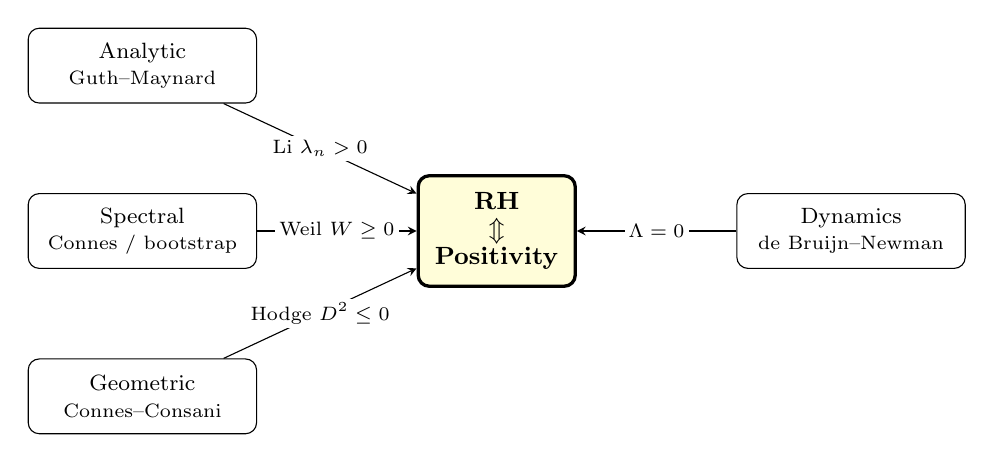
\begin{tikzpicture}[
   box/.style={draw,rounded corners,align=center,font=\footnotesize,inner sep=4pt,minimum width=2.9cm,minimum height=0.95cm},
   ctrbox/.style={draw,very thick,fill=yellow!15,rounded corners,align=center,font=\small,inner sep=6pt},
   lab/.style={font=\scriptsize,fill=white,inner sep=1.5pt}]
   \node[ctrbox] (P) at (0,0) {\textbf{RH}\\[-1pt]$\Updownarrow$\\[-1pt]\textbf{Positivity}};
   \node[box] (A) at (-4.5,2.1) {Analytic\\\scriptsize Guth--Maynard};
   \node[box] (S) at (-4.5,0)   {Spectral\\\scriptsize Connes / bootstrap};
   \node[box] (G) at (-4.5,-2.1){Geometric\\\scriptsize Connes--Consani};
   \node[box] (D) at (4.5,0)    {Dynamics\\\scriptsize de Bruijn--Newman};
   \draw[->,>=stealth] (A) -- node[lab]{Li $\lambda_n>0$} (P);
   \draw[->,>=stealth] (S) -- node[lab]{Weil $W\ge 0$} (P);
   \draw[->,>=stealth] (G) -- node[lab]{Hodge $D^2\le 0$} (P);
   \draw[->,>=stealth] (D) -- node[lab]{$\Lambda=0$} (P);
\end{tikzpicture}
\caption{The convergence of approaches onto a positivity condition. Each front reduces the Riemann Hypothesis to the (strict) positivity or definiteness of a mathematical object: the Li coefficients $\lambda_n$, the Weil functional $W$, an intersection form (Hodge/Castelnuovo--Severi $D^2\le0$), and---dynamically---the de Bruijn--Newman constant $\Lambda=0$. The first two are \emph{proved} equivalent to RH; the third is a geometric program; $\Lambda=0$ is a theorem-level reformulation (with $\Lambda\ge0$ proved by Rodgers--Tao). The positivities live in different categories and are not known to be equivalent to one another.}
\label{fig:positivity}
\end{figure}

To maintain precision, we distinguish three levels of rigor among these positivity conditions:
\begin{enumerate}[label=(\roman*)]
\item \textbf{Rigorous equivalences.} Li's criterion ($\lambda_n > 0$ for all $n$) and Weil positivity ($W(h * \tilde{h}) \ge 0$ for all admissible $h$) are each \emph{proved equivalent} to RH. The Lagarias theorem (Section~\ref{sec:li}) provides a precise mathematical bridge between these two: the Li coefficients are evaluations of the Weil functional. These are not merely suggestive---they are theorems.
\item \textbf{Operator-theoretic programs.} The Connes trace formula and the prolate wave operator program reduce RH to establishing Weil positivity in the adelic setting. This is a precise mathematical program with a clearly identified target, but the target (global Weil positivity) has not been reached.
\item \textbf{Physics-inspired analogies.} The CFT unitarity condition ($d(\Delta) \ge 0$) and the Hodge Index Theorem on the arithmetic square provide \emph{structural analogues} of positivity in their respective domains. These are reformulations and sources of constraints, but neither has yet been shown to rigorously imply RH.
\end{enumerate}

At a deeper level, the positivity conditions in Table~\ref{tab:positivity} can be interpreted through a unifying dynamical lens: in each framework, the Riemann Hypothesis asserts that \emph{constructive interference dominates destructive interference} within a structured arithmetic system. In the analytic setting, this manifests as the geometric control of wave packet overlaps; in the spectral setting, as the reality of eigenvalues (equivalently, the absence of growing modes); in the CFT context, as the absence of negative-norm states; and in the geometric setting, as the definite signature of an intersection form. The positivity conditions are, in each case, the mathematical expression of a stable oscillatory regime.

This conceptual convergence strongly suggests that any successful proof will involve establishing a positivity structure in one of these frameworks---a structural guarantee that an underlying arithmetic, geometric, or physical state space possesses a strictly positive metric. Whether this positivity is ultimately derived from the geometric curvature of time-frequency wave packets, the intersection theory of the sphere spectrum, or the reflection positivity of a quantum field theory remains the defining question for the next decade of research. It is also possible that RH holds for fundamentally different reasons in different frameworks, and that the apparent convergence to positivity is a consequence rather than a cause.

Conversely, it is worth noting why a \emph{counterexample} to RH is also considered extremely unlikely. A zero off the critical line would simultaneously violate: the Li positivity condition ($\lambda_n < 0$ for some $n$), the Weil positivity condition, the random matrix predictions for zero spacings (contradicting extensive numerical evidence at heights up to $10^{22}$), and the rigorous computational verification for the first $1.3 \times 10^{13}$ zeros (Platt--Trudgian). The consistency of RH across all of these independent frameworks---analytic, spectral, probabilistic, and computational---provides the strongest collective evidence for any open conjecture in mathematics.

%% ======================================================================
\section{Potential Paths Forward}\label{sec:paths}
%% ======================================================================

Based on the developments surveyed above, we identify three directions that appear most promising for future progress.

\subsection{The Algebro-Geometric Path}\label{sec:path-geom}

Complete the Weil strategy for $\mathbb{Z}$ by developing intersection theory on the arithmetic square and proving the Hodge Index Theorem in the tropical/topos-theoretic setting. This is the only approach that would provide a \emph{structural} explanation for RH, deriving it as a consequence of the geometry of $\operatorname{Spec}(\mathbb{Z})$. The 2024 Riemann--Roch theorem suggests the formalism is approaching maturity, but the obstacles identified in Section~\ref{sec:cc-critique} remain substantial.

\textbf{Specific milestones needed:}
\begin{enumerate}[label=(\roman*)]
\item Construct a well-defined intersection theory on the product $\operatorname{Spec}(\mathbb{Z}) \times_{\mathbb{S}} \operatorname{Spec}(\mathbb{Z})$, including a notion of intersection number for divisors on this ``surface.''
\item Develop a Hodge theory (or substitute) in the tropical/topos-theoretic setting that provides the positivity properties needed for the Hodge Index Theorem.
\item Identify the analogue of the Frobenius correspondence $\Gamma_{\operatorname{Fr}} \subset C \times C$ for $\operatorname{Spec}(\mathbb{Z})$ and compute its self-intersection in the new framework.
\end{enumerate}

Each of these steps presents fundamental conceptual challenges, not merely technical ones. In particular, step (ii) requires a notion of ``positivity'' in tropical geometry that does not yet exist in the required generality.

\subsection{The Analytic Path}\label{sec:path-analytic}

Refine the Guth--Maynard estimates to obtain progressively stronger density bounds, and combine these with advances in mollifier technology and moment estimates to increase the proven proportion of zeros on the critical line. This path uses established techniques and does not rely on finding new conceptual frameworks.

\textbf{Concrete targets:}
\begin{enumerate}[label=(\roman*)]
\item Extend the Guth--Maynard large value estimates to the full range $1/2 < \sigma < 1$, potentially establishing the \emph{density hypothesis} $N(\sigma, T) \ll T^{2(1-\sigma) + \varepsilon}$, which remains one of the central open problems in analytic number theory.
\item Increase the proven proportion of zeros on the critical line beyond the current 41.67\%. Breaking the 50\% barrier would be a landmark achievement, as it would require fundamentally new ideas beyond the current mollifier technology.
\item Improve estimates for primes in short intervals, possibly reaching the conjectured optimal exponent $\theta = 1/2 + \varepsilon$ (which follows from RH).
\end{enumerate}

The ultimate limitation of the analytic path is clear: density estimates can prove that exceptions are rare, not that they are absent. To prove $N(\sigma, T) = 0$ for $\sigma > 1/2$ requires a qualitative leap beyond what measure-theoretic bounds can provide. Nevertheless, analytic advances have historically driven progress on the problem and are likely to continue doing so.

\subsection{The Spectral-Bootstrap Path}\label{sec:path-spectral}

Exploit the connection between $\zeta(s)$ and conformal field theory established by the scalar modular bootstrap. If the constraints of unitarity and modular invariance can be shown to be sufficiently restrictive---for instance, by proving the existence of a specific CFT whose consistency requires all zeta zeros to be on the critical line---this would yield a proof of RH as a consequence of physical consistency.

\textbf{Key questions:}
\begin{enumerate}[label=(\roman*)]
\item Does there exist a unitary 2d CFT with $U(1)^c$ symmetry whose scalar spectrum is directly determined by the non-trivial zeros of $\zeta(s)$? If so, the unitarity of the theory would immediately imply RH.
\item Can the numerical bootstrap methods (semidefinite programming) be used to derive rigorous bounds on $\zeta(s)$ that go beyond what is achievable by purely analytic means?
\item What is the precise relationship between the crossing equation of Benjamin--Chang and the Weil positivity condition of Connes? Both are ``positivity conditions,'' and a direct connection between them would unify the spectral and geometric approaches.
\end{enumerate}

This path is the most speculative of the three, but it brings powerful computational and theoretical tools from mathematical physics into contact with the problem.

\subsection{A Computational Probe of Weil Positivity}\label{sec:weil-probe}

The reformulations of Section~\ref{sec:equiv} and the synthesis of Section~\ref{sec:synthesis} both identify \emph{Weil positivity}---the condition $W(h * \tilde h) \ge 0$ for all admissible test functions $h$, where $W$ is the Weil functional of the explicit formula---as one of the two reformulations \emph{proved} equivalent to RH. This invites a concrete experimental program: realize the Weil functional as a finite quadratic form on an explicit, localized family of test functions, and probe its positivity numerically against functions that satisfy RH and against functions that violate it.

Concretely, one fixes a localized basis---for instance Hermite--Gauss functions $\{\varphi_j\}$ centered at a height $T_0$ with width $\sigma$ and dimension $J$---and assembles the Gram matrix $Q_{jk} = W(\varphi_j * \tilde\varphi_k)$ of the Weil functional in that basis, evaluated through the explicit formula (zeros on one side; archimedean, polar, and prime-power contributions on the other). The smallest eigenvalue $\lambda_{\min}(Q)$ then serves as a localized detector: an off-critical zero near $T_0$ should drive $\lambda_{\min}(Q)$ negative, while an $L$-function obeying its Riemann hypothesis should keep $Q$ positive semidefinite. Computational work of the present author reports that, when the arithmetic side is included in full, this construction (i) flags the off-critical zeros of the Davenport--Heilbronn function (Section~\ref{sec:whyhard}) through a strongly negative $\lambda_{\min}$, with no false positives across genuine $L$-functions (the Riemann $\zeta$, a Dirichlet $L(s,\chi)$, and a degree-two modular $L$-function); (ii) exhibits negativity that is \emph{intrinsically local}, appearing only when $T_0$ lies near the off-critical zero; and (iii) scales quadratically in the displacement of a zero off the line, with sensitivity amplifying super-polynomially in the basis dimension $J$.

The epistemic status of such a probe must be stated carefully, and it mirrors the broader lesson of this survey. The \emph{detector direction}---an off-critical zero forces $\lambda_{\min}(Q) < 0$---is the accessible half of Weil's criterion and can be made into a rigorous, quantitative statement. The \emph{converse}---global positivity $\lambda_{\min}(Q) \ge 0$ across all centers, widths, and dimensions---is Weil positivity itself, hence equivalent to RH, and no finite computation can establish it (finite-dimensional positivity does not imply the infinite-dimensional condition). The value of the experimental probe is therefore not evidential but structural: it makes the Weil positivity condition computationally concrete, it isolates the precise analytic obstruction separating a \emph{detector} from a \emph{theorem}---a uniform-in-basis control of the truncation error between the finite form $Q$ and the full Weil functional---and it furnishes a fast falsifier against which candidate positivity structures (de Branges spaces, the Connes trace, the bootstrap functional) can be tested before substantial theoretical investment. In this sense the computational probe is a microcosm of the positivity convergence described in Section~\ref{sec:synthesis}: it confirms, in an explicit and reproducible setting, that the entire difficulty of RH is concentrated in establishing a single positivity uniformly.

\subsection{A Note on Interaction Between Approaches}\label{sec:interaction}

It is worth emphasizing that the three paths described above are not mutually exclusive. A proof of RH may well combine elements from multiple approaches. For example:
\begin{itemize}
\item The analytic estimates of Guth--Maynard could provide the ``hard analysis'' component of a proof whose structural framework comes from the geometric or spectral approach.
\item The Weil positivity condition, which appears in both the Connes trace formula and the Connes--Consani geometric program, could be established using techniques from harmonic analysis (as in the zero density estimates) rather than from algebraic geometry.
\item The random matrix predictions of Keating--Snaith, which originate in the spectral approach, have already guided the development of analytic techniques (mollifiers, moment calculations) and could continue to do so.
\end{itemize}

The history of the Weil conjectures is instructive: Deligne's proof of the last Weil conjecture (1974) \cite{deligne1974} used methods (\'etale cohomology, the Lefschetz trace formula) that Weil himself did not have access to, and the proof looked quite different from what Weil had envisioned. A proof of RH for $\mathbb{Q}$ may similarly require tools that do not yet exist, or may combine existing tools in unexpected ways.

%% ======================================================================
\section*{Concluding Remarks}\label{sec:conclusion}
%% ======================================================================

The Riemann Hypothesis has been open for over 165 years. During this time, it has stimulated the development of large portions of analytic number theory, algebraic geometry, random matrix theory, and noncommutative geometry. The progress surveyed here---particularly the Guth--Maynard breakthrough on zero density, the Connes--Consani Riemann--Roch theorem, and the emerging connections to conformal field theory---represents a significant advance in our understanding of the problem, even if a proof remains out of reach.

We close with remarks on scope and on directions accessible to researchers entering the field.

\textbf{Scope.} This survey has focused on the Riemann Hypothesis for the Riemann zeta function $\zeta(s)$. The \emph{Generalized Riemann Hypothesis} (GRH), which asserts that all non-trivial zeros of Dirichlet $L$-functions $L(s, \chi)$ lie on $\operatorname{Re}(s) = 1/2$, and the broader \emph{Grand Riemann Hypothesis} for automorphic $L$-functions, are equally important conjectures with far-reaching consequences in algebraic number theory, arithmetic geometry, and cryptography. Many of the approaches discussed here---particularly the spectral and geometric ones---are expected to apply to these generalizations as well. Indeed, a proof of RH that does not generalize to at least Dirichlet $L$-functions would be considered surprising, and most researchers expect that the correct proof will establish GRH simultaneously. For a discussion of the consequences of GRH, see Iwaniec--Kowalski \cite{iwaniec2004}.

\textbf{Accessible open problems.} For researchers entering the field, we highlight several concrete problems that are adjacent to RH and potentially tractable within the next five to ten years:
\begin{enumerate}[label=(\roman*)]
\item \textbf{Extending Guth--Maynard.} Extend the large value estimates for Dirichlet polynomials to new ranges of $\sigma$, or adapt the wave packet framework to $L$-functions beyond $\zeta(s)$. The ANTEDB infrastructure \cite{tao2025} provides a systematic way to propagate such improvements.
\item \textbf{Breaking the 50\% barrier.} Prove that more than 50\% of zeros lie on the critical line. This is widely regarded as requiring qualitatively new mollifier techniques (``two-piece'' mollifiers, or techniques that circumvent the parity barrier).
\item \textbf{Fyodorov--Hiary--Keating conjecture.} Prove the leading-order prediction for the maximum of $|\zeta(1/2 + it)|$ in intervals of bounded length. Partial results exist, but the sharp constant remains open.
\item \textbf{Intersection theory over $\mathbb{S}$.} Develop a rigorous intersection pairing on $\operatorname{Spec}(\mathbb{Z}) \times_{\mathbb{S}} \operatorname{Spec}(\mathbb{Z})$ and compute explicit intersection numbers for natural divisors. Even partial results would represent a major advance in absolute arithmetic geometry.
\item \textbf{Bootstrap bounds.} Use the numerical conformal bootstrap (semidefinite programming) to derive rigorous arithmetic bounds from the Benjamin--Chang crossing equation that go beyond what is currently achievable by purely analytic means.
\end{enumerate}

%% ======================================================================
%% BIBLIOGRAPHY
%% ======================================================================

\begin{thebibliography}{64}

\bibitem{berry1999}
M.\,V. Berry and J.\,P. Keating,
\textit{The Riemann zeros and eigenvalue asymptotics},
SIAM Review \textbf{41} (1999), no.~2, 236--266.
\textsc{doi:} \href{https://doi.org/10.1137/S0036144598347497}{10.1137/S0036144598347497}.

\bibitem{benjamin2022}
N. Benjamin and C. Chang,
\textit{Scalar modular bootstrap and zeros of the Riemann zeta function},
J. High Energy Phys. \textbf{2022}, no.~11, Paper No.~143.
\textsc{doi:} \href{https://doi.org/10.1007/JHEP11(2022)143}{10.1007/JHEP11(2022)143}.

\bibitem{bombieri2000}
E. Bombieri,
\textit{Problems of the Millennium: The Riemann Hypothesis},
Clay Mathematics Institute (2000).
\url{https://www.claymath.org/wp-content/uploads/2022/05/riemann.pdf}

\bibitem{bost1995}
J.-B. Bost and A. Connes,
\textit{Hecke algebras, type III factors and phase transitions with spontaneous symmetry breaking in number theory},
Selecta Math. (N.S.) \textbf{1} (1995), no.~3, 411--457.
\url{https://alainconnes.org/wp-content/uploads/bostconnesscan.pdf}

\bibitem{bourgain2016}
J. Bourgain, C. Demeter, and L. Guth,
\textit{Proof of the main conjecture in Vinogradov's mean value theorem for degrees higher than three},
Ann. of Math. (2) \textbf{184} (2016), no.~2, 633--682.
\textsc{doi:} \href{https://doi.org/10.4007/annals.2016.184.2.7}{10.4007/annals.2016.184.2.7}.

\bibitem{connes1999}
A. Connes,
\textit{Trace formula in noncommutative geometry and the zeros of the Riemann zeta function},
Selecta Math. (N.S.) \textbf{5} (1999), no.~1, 29--106.
\url{https://arxiv.org/abs/math/9811068}

\bibitem{connes2019}
A. Connes and C. Consani,
\textit{The Scaling Site},
J. Reine Angew. Math. \textbf{755} (2019), 1--43.
\url{https://arxiv.org/abs/1507.05818}

\bibitem{connes2024}
A. Connes and C. Consani,
\textit{Riemann-Roch for the ring $\mathbb{Z}$},
C. R. Math. Acad. Sci. Paris \textbf{362} (2024), 1727--1732.
\url{https://arxiv.org/abs/2306.00456}

\bibitem{conrey1989}
J.\,B. Conrey,
\textit{More than two fifths of the zeros of the Riemann zeta function are on the critical line},
J. Reine Angew. Math. \textbf{399} (1989), 1--26.
\textsc{doi:} \href{https://doi.org/10.1515/crll.1989.399.1}{10.1515/crll.1989.399.1}.

\bibitem{conrey2003}
J.\,B. Conrey,
\textit{The Riemann Hypothesis},
Notices Amer. Math. Soc. \textbf{50} (2003), no.~3, 341--353.
\url{https://www.ams.org/notices/200303/fea-conrey-web.pdf}

\bibitem{deligne1974}
P. Deligne,
\textit{La conjecture de Weil. I},
Publ. Math. Inst. Hautes \'Etudes Sci. \textbf{43} (1974), 273--307.
\textsc{doi:} \href{https://doi.org/10.1007/BF02684373}{10.1007/BF02684373}.

\bibitem{edwards1974}
H.\,M. Edwards,
\textit{Riemann's Zeta Function},
Academic Press, 1974; Dover reprint, 2001.
\url{http://www.stat.ucla.edu/~ywu/Riemann.pdf}

\bibitem{guth2024}
L. Guth and J. Maynard,
\textit{New large value estimates for Dirichlet polynomials},
arXiv preprint arXiv:2405.20552 (2024).
\url{https://arxiv.org/abs/2405.20552}

\bibitem{hiary2012}
G.\,A. Hiary and A.\,M. Odlyzko,
\textit{The zeta function on the critical line: numerical evidence for moments and random matrix theory models},
Math. Comp. \textbf{81} (2012), no.~279, 1723--1752.
\textsc{doi:} \href{https://doi.org/10.1090/S0025-5718-2011-02573-1}{10.1090/S0025-5718-2011-02573-1}.

\bibitem{iwaniec2004}
H. Iwaniec and E. Kowalski,
\textit{Analytic Number Theory},
Amer. Math. Soc. Colloq. Publ., vol.~53, Amer. Math. Soc., Providence, RI, 2004.
\url{https://bookstore.ams.org/coll-53/}

\bibitem{keating2000}
J.\,P. Keating and N.\,C. Snaith,
\textit{Random matrix theory and $\zeta(1/2+it)$},
Comm. Math. Phys. \textbf{214} (2000), no.~1, 57--89.
\textsc{doi:} \href{https://doi.org/10.1007/s002200000261}{10.1007/s002200000261}.

\bibitem{lagarias2005}
J.\,C. Lagarias,
\textit{Li coefficients for automorphic $L$-functions},
Ann. Inst. Fourier (Grenoble) \textbf{57} (2007), no.~5, 1689--1740.
\textsc{doi:} \href{https://doi.org/10.5802/aif.2311}{10.5802/aif.2311}.

\bibitem{levinson1974}
N. Levinson,
\textit{More than one third of zeros of Riemann's zeta-function are on $\sigma = 1/2$},
Adv. Math. \textbf{13} (1974), 383--436.
\textsc{doi:} \href{https://doi.org/10.1016/0001-8708(74)90074-7}{10.1016/0001-8708(74)90074-7}.

\bibitem{li1997}
X.-J. Li,
\textit{The positivity of a sequence of numbers and the Riemann hypothesis},
J. Number Theory \textbf{65} (1997), no.~2, 325--333.
\textsc{doi:} \href{https://doi.org/10.1006/jnth.1997.2137}{10.1006/jnth.1997.2137}.

\bibitem{montgomery1973}
H.\,L. Montgomery,
\textit{The pair correlation of zeros of the zeta function},
Analytic Number Theory (Proc. Sympos. Pure Math., Vol.~XXIV, St. Louis, 1972),
Amer. Math. Soc., 1973, pp.~181--193.
\url{https://websites.umich.edu/~hlm/paircor1.pdf}

\bibitem{mossinghoff2024}
M.\,J. Mossinghoff, T.\,S. Trudgian, and A. Yang,
\textit{Explicit zero-free regions for the Riemann zeta-function},
Res. Number Theory \textbf{10} (2024), Paper No.~11.
\textsc{doi:} \href{https://doi.org/10.1007/s40993-023-00498-y}{10.1007/s40993-023-00498-y}.

\bibitem{platt2021}
D.\,J. Platt and T.\,S. Trudgian,
\textit{The Riemann hypothesis is true up to $3 \times 10^{12}$},
Bull. London Math. Soc. \textbf{53} (2021), no.~3, 792--797.
\textsc{doi:} \href{https://doi.org/10.1112/blms.12460}{10.1112/blms.12460}.

\bibitem{pratt2020}
K. Pratt, N. Robles, A. Zaharescu, and D. Zeindler,
\textit{More than five-twelfths of the zeros of $\zeta$ are on the critical line},
Res. Math. Sci. \textbf{7} (2020), Paper No.~2.
\textsc{doi:} \href{https://doi.org/10.1007/s40687-019-0199-8}{10.1007/s40687-019-0199-8}.

\bibitem{radziwill2018}
M. Radziwi\l\l{} and K. Soundararajan,
\textit{Moments and distribution of central $L$-values of quadratic twists of elliptic curves}, (2014).
\url{https://arxiv.org/abs/1403.7067}

\bibitem{sarnak2004}
P. Sarnak,
\textit{Problems of the Millennium: The Riemann Hypothesis},
2004.
\url{https://www.claymath.org/library/annual_report/ar2004/04report_sarnak.pdf}

\bibitem{selberg1942}
A. Selberg,
\textit{On the zeros of Riemann's zeta-function},
Skr. Norske Vid.-Akad. Oslo I \textbf{10} (1942), 1--59.
\url{https://sites.math.rutgers.edu/~zeilberg/EM18/selberg1942.pdf}

\bibitem{titchmarsh1986}
E.\,C. Titchmarsh,
\textit{The Theory of the Riemann Zeta-Function},
2nd ed. (revised by D.\,R. Heath-Brown),
Oxford Univ. Press, 1986.
\url{https://sites.math.rutgers.edu/~zeilberg/EM18/TitchmarshZeta.pdf}

\bibitem{weil1948}
A. Weil,
\textit{Sur les courbes alg\'ebriques et les vari\'et\'es qui s'en d\'eduisent},
Actualit\'es Sci. Ind., no.~1041,
Hermann, Paris, 1948.
\url{https://denise.vella.chemla.free.fr/Weil-courbes-varietes.pdf}

\bibitem{wooley2016}
T.\,D. Wooley,
\textit{The cubic case of the main conjecture in Vinogradov's mean value theorem},
Adv. Math. \textbf{294} (2016), 532--561.
\textsc{doi:} \href{https://doi.org/10.1016/j.aim.2016.02.033}{10.1016/j.aim.2016.02.033}.

\bibitem{riemann1859}
B. Riemann,
\textit{\"Ueber die Anzahl der Primzahlen unter einer gegebenen Gr\"osse},
Monatsberichte der Berliner Akademie (1859), 671--680.
\url{https://www.claymath.org/library/historical/riemann/german/Zeta.pdf}

\bibitem{hardy1914}
G.\,H. Hardy,
\textit{Sur les z\'eros de la fonction $\zeta(s)$ de Riemann},
C. R. Acad. Sci. Paris \textbf{158} (1914), 1012--1014.
\url{https://www.scirp.org/reference/referencespapers?referenceid=3196980}

\bibitem{rudnick1996}
Z. Rudnick and P. Sarnak,
\textit{Zeros of principal $L$-functions and random matrix theory},
Duke Math. J. \textbf{81} (1996), no.~2, 269--322.
\textsc{doi:} \href{https://doi.org/10.1215/S0012-7094-96-08115-6}{10.1215/S0012-7094-96-08115-6}.

\bibitem{conrey2008}
J.\,B. Conrey, D.\,W. Farmer, and M.\,R. Zirnbauer,
\textit{Autocorrelation of ratios of $L$-functions},
Commun. Number Theory Phys. \textbf{2} (2008), no.~3, 593--636.
\textsc{doi:} \href{https://doi.org/10.4310/CNTP.2008.v2.n3.a4}{10.4310/CNTP.2008.v2.n3.a4}.

\bibitem{huxley1972}
M.\,N. Huxley,
\textit{On the difference between consecutive primes},
Invent. Math. \textbf{15} (1972), 164--170.
\textsc{doi:} \href{https://doi.org/10.1007/BF01418933}{10.1007/BF01418933}.

\bibitem{ingham1940}
A.\,E. Ingham,
\textit{On the estimation of $N(\sigma, T)$},
Quart. J. Math. Oxford Ser. \textbf{11} (1940), 291--292.
\url{https://academic.oup.com/qjmath/article-abstract/os-11/1/201/1574975?redirectedFrom=fulltext&login=false}

\bibitem{delavallee1899}
Ch.-J. de la Vall\'ee Poussin,
\textit{Sur la fonction $\zeta(s)$ de Riemann et le nombre des nombres premiers inf\'erieurs \`a une limite donn\'ee},
M\'em. Couronn\'es et Autres M\'em. Acad. Roy. Sci. Belgique \textbf{59} (1899).
\url{https://www.persee.fr/doc/marb_0770-8459_1899_num_59_1_2449}

\bibitem{conrey2005}
J.\,B. Conrey and N.\,C. Snaith,
\textit{Applications of the $L$-functions ratios conjectures},
Proc. London Math. Soc. (3) \textbf{94} (2007), no.~3, 594--646.
\textsc{doi:} \href{https://doi.org/10.1112/plms/pdl021}{10.1112/plms/pdl021}.

\bibitem{odlyzko1987}
A.\,M. Odlyzko,
\textit{On the distribution of spacings between zeros of the zeta function},
Math. Comp. \textbf{48} (1987), no.~177, 273--308.
\textsc{doi:} \href{https://doi.org/10.1090/S0025-5718-1987-0866115-0}{10.1090/S0025-5718-1987-0866115-0}.

\bibitem{korobov1958}
N.\,M. Korobov,
\textit{Estimates of trigonometric sums and their applications},
Uspekhi Mat. Nauk \textbf{13} (1958), no.~4, 185--192.
\url{https://www.mathnet.ru/php/archive.phtml?wshow=paper&jrnid=rm&paperid=7458&option_lang=eng}

\bibitem{tao2025}
T. Tao, T.\,S. Trudgian, and A. Yang,
\textit{New exponent pairs, zero density estimates, and zero additive energy estimates: a systematic approach},
Math. Comp. (2025).
\textsc{doi:} \href{https://doi.org/10.1090/mcom/4138}{10.1090/mcom/4138}.

\bibitem{gafni2025}
A. Gafni and T. Tao,
\textit{Bounding the number of exceptional intervals in the prime number theorem in short intervals},
 (2025).
\url{https://arxiv.org/abs/2505.24017}

\bibitem{hieu2025}
L.\,D. Hieu,
\textit{Arithmetic progressions of primes in short intervals beyond the $17/30$ barrier},
 (2025).
\url{https://arxiv.org/abs/2509.04883}

\bibitem{leclair2024}
A. LeClair and G. Mussardo,
\textit{Generalized Riemann hypothesis, time series and normal distributions}, (2018).
\url{https://arxiv.org/abs/1809.06158}.

\bibitem{connes2024b}
A. Connes, C. Consani, and H. Moscovici,
\textit{Zeta zeros and prolate wave operators},
Ann. Funct. Anal. \textbf{15} (2024), no.~4, Paper No.~71.
\textsc{doi:} \href{https://doi.org/10.1007/s43034-024-00388-z}{10.1007/s43034-024-00388-z}.

\bibitem{soundararajan2008}
K. Soundararajan,
\textit{Extreme values of zeta and $L$-functions},
Math. Ann. \textbf{342} (2008), no.~2, 467--486.
\textsc{doi:} \href{https://doi.org/10.1007/s00208-008-0243-2}{10.1007/s00208-008-0243-2}.

\bibitem{bondarenko2017}
A. Bondarenko and K. Seip,
\textit{Large greatest common divisor sums and extreme values of the Riemann zeta function},
Duke Math. J. \textbf{166} (2017), no.~9, 1685--1701.
\textsc{doi:} \href{https://doi.org/10.1215/00127094-0000005X}{10.1215/00127094-0000005X}.

\bibitem{fyodorov2012}
Y.\,V. Fyodorov, G.\,A. Hiary, and J.\,P. Keating,
\textit{Freezing transition, characteristic polynomials of random matrices, and the Riemann zeta function},
Phys. Rev. Lett. \textbf{108} (2012), 170601.
\textsc{doi:} \href{https://doi.org/10.1103/PhysRevLett.108.170601}{10.1103/PhysRevLett.108.170601}.

\bibitem{voronin1975}
S.\,M. Voronin,
\textit{Theorem on the ``universality'' of the Riemann zeta-function}, (1975).
\textsc{doi:} \href{https://doi.org/10.1070/IM1975v009n03ABEH001485}{10.1070/IM1975v009n03ABEH001485}.

\bibitem{rhodes2014}
R. Rhodes and V. Vargas,
\textit{Gaussian multiplicative chaos and applications: a review},
Probab. Surv. \textbf{11} (2014), 315--392.
\textsc{doi:} \href{https://doi.org/10.1214/13-PS218}{10.1214/13-PS218}.

\bibitem{saksman2020}
E. Saksman and C. Webb,
\textit{The Riemann zeta function and Gaussian multiplicative chaos: statistics on the critical line},
Ann. Probab. \textbf{48} (2020), no.~6, 2680--2754.
\textsc{doi:} \href{https://doi.org/10.1214/20-AOP1433}{10.1214/20-AOP1433}.

\bibitem{bellotti2023}
C. Bellotti,
\textit{Explicit zero density estimate near unity},
preprint (2023).
\url{https://arxiv.org/abs/2311.05136}

\bibitem{connes2023}
A. Connes and C. Consani,
\textit{BC-system, absolute cyclotomy and the quantized calculus},
EMS Surv. Math. Sci. \textbf{9} (2023), no.~2, 447--475.
\textsc{doi:} \href{https://doi.org/10.4171/emss/64}{10.4171/EMSS/64}.

\bibitem{connes2025}
A. Connes, C. Consani, and H. Moscovici,
\textit{Zeta spectral triples},
preprint (2025).
\url{https://arxiv.org/abs/2511.22755}

\bibitem{connes2026}
A. Connes,
\textit{The Riemann Hypothesis: past, present and a letter through time},
preprint (2026).
\url{https://arxiv.org/abs/2602.04022}

\bibitem{amberger2025}
V. Amberger,
\textit{Bounding the integral of the argument of the Riemann zeta function},
preprint (2025).
\url{https://arxiv.org/abs/2512.23064}

\bibitem{li2024}
R. Li,
\textit{Primes in almost all short intervals},
preprint (2024).
\url{https://arxiv.org/abs/2407.05651}

\bibitem{debruijn1950}
N.\,G. de Bruijn,
\textit{The roots of trigonometric integrals},
Duke Math. J. \textbf{17} (1950), 197--226.
\textsc{doi:} \href{https://doi.org/10.1215/S0012-7094-50-01720-0}{10.1215/S0012-7094-50-01720-0}.

\bibitem{newman1976}
C.\,M. Newman,
\textit{Fourier transforms with only real zeros},
Proc. Amer. Math. Soc. \textbf{61} (1976), no.~2, 245--251.
\textsc{doi:} \href{https://doi.org/10.1090/S0002-9939-1976-0434982-5}{10.1090/S0002-9939-1976-0434982-5}.

\bibitem{rodgers2020}
B. Rodgers and T. Tao,
\textit{The de Bruijn--Newman constant is non-negative},
Forum Math. Pi \textbf{8} (2020), e6, 62 pp.
\textsc{doi:} \href{https://doi.org/10.1017/fmp.2020.6}{10.1017/fmp.2020.6}.

\bibitem{polymath2019}
D.\,H.\,J. Polymath,
\textit{Effective approximation of heat flow evolution of the Riemann $\xi$ function, and a new upper bound for the de Bruijn--Newman constant},
Res. Math. Sci. \textbf{6} (2019), no.~3, Paper No.~31.
\textsc{doi:} \href{https://doi.org/10.1007/s40687-019-0193-1}{10.1007/s40687-019-0193-1}.

\bibitem{beurling1955}
A. Beurling,
\textit{A closure problem related to the Riemann zeta-function},
Proc. Nat. Acad. Sci. U.S.A. \textbf{41} (1955), no.~5, 312--314.
\textsc{doi:} \href{https://doi.org/10.1073/pnas.41.5.312}{10.1073/pnas.41.5.312}.

\bibitem{baezduarte2003}
L. B\'aez-Duarte,
\textit{A strengthening of the Nyman--Beurling criterion for the Riemann hypothesis},
Atti Accad. Naz. Lincei Cl. Sci. Fis. Mat. Natur. Rend. Lincei (9) Mat. Appl. \textbf{14} (2003), no.~1, 5--11.
\url{https://arxiv.org/abs/math/0202141}

\end{thebibliography}

\end{document}
